% Options for packages loaded elsewhere
\PassOptionsToPackage{unicode}{hyperref}
\PassOptionsToPackage{hyphens}{url}
\PassOptionsToPackage{dvipsnames,svgnames,x11names}{xcolor}
%
\documentclass[
]{article}

\usepackage{amsmath,amssymb}
\usepackage{iftex}
\ifPDFTeX
  \usepackage[T1]{fontenc}
  \usepackage[utf8]{inputenc}
  \usepackage{textcomp} % provide euro and other symbols
\else % if luatex or xetex
  \usepackage{unicode-math}
  \defaultfontfeatures{Scale=MatchLowercase}
  \defaultfontfeatures[\rmfamily]{Ligatures=TeX,Scale=1}
\fi
\usepackage[]{libertinus}
\ifPDFTeX\else  
    % xetex/luatex font selection
\fi
% Use upquote if available, for straight quotes in verbatim environments
\IfFileExists{upquote.sty}{\usepackage{upquote}}{}
\IfFileExists{microtype.sty}{% use microtype if available
  \usepackage[]{microtype}
  \UseMicrotypeSet[protrusion]{basicmath} % disable protrusion for tt fonts
}{}
\makeatletter
\@ifundefined{KOMAClassName}{% if non-KOMA class
  \IfFileExists{parskip.sty}{%
    \usepackage{parskip}
  }{% else
    \setlength{\parindent}{0pt}
    \setlength{\parskip}{6pt plus 2pt minus 1pt}}
}{% if KOMA class
  \KOMAoptions{parskip=half}}
\makeatother
\usepackage{xcolor}
\setlength{\emergencystretch}{3em} % prevent overfull lines
\setcounter{secnumdepth}{5}
% Make \paragraph and \subparagraph free-standing
\ifx\paragraph\undefined\else
  \let\oldparagraph\paragraph
  \renewcommand{\paragraph}[1]{\oldparagraph{#1}\mbox{}}
\fi
\ifx\subparagraph\undefined\else
  \let\oldsubparagraph\subparagraph
  \renewcommand{\subparagraph}[1]{\oldsubparagraph{#1}\mbox{}}
\fi

\usepackage{color}
\usepackage{fancyvrb}
\newcommand{\VerbBar}{|}
\newcommand{\VERB}{\Verb[commandchars=\\\{\}]}
\DefineVerbatimEnvironment{Highlighting}{Verbatim}{commandchars=\\\{\}}
% Add ',fontsize=\small' for more characters per line
\newenvironment{Shaded}{}{}
\newcommand{\AlertTok}[1]{\textcolor[rgb]{1.00,0.33,0.33}{\textbf{#1}}}
\newcommand{\AnnotationTok}[1]{\textcolor[rgb]{0.42,0.45,0.49}{#1}}
\newcommand{\AttributeTok}[1]{\textcolor[rgb]{0.84,0.23,0.29}{#1}}
\newcommand{\BaseNTok}[1]{\textcolor[rgb]{0.00,0.36,0.77}{#1}}
\newcommand{\BuiltInTok}[1]{\textcolor[rgb]{0.84,0.23,0.29}{#1}}
\newcommand{\CharTok}[1]{\textcolor[rgb]{0.01,0.18,0.38}{#1}}
\newcommand{\CommentTok}[1]{\textcolor[rgb]{0.42,0.45,0.49}{#1}}
\newcommand{\CommentVarTok}[1]{\textcolor[rgb]{0.42,0.45,0.49}{#1}}
\newcommand{\ConstantTok}[1]{\textcolor[rgb]{0.00,0.36,0.77}{#1}}
\newcommand{\ControlFlowTok}[1]{\textcolor[rgb]{0.84,0.23,0.29}{#1}}
\newcommand{\DataTypeTok}[1]{\textcolor[rgb]{0.84,0.23,0.29}{#1}}
\newcommand{\DecValTok}[1]{\textcolor[rgb]{0.00,0.36,0.77}{#1}}
\newcommand{\DocumentationTok}[1]{\textcolor[rgb]{0.42,0.45,0.49}{#1}}
\newcommand{\ErrorTok}[1]{\textcolor[rgb]{1.00,0.33,0.33}{\underline{#1}}}
\newcommand{\ExtensionTok}[1]{\textcolor[rgb]{0.84,0.23,0.29}{\textbf{#1}}}
\newcommand{\FloatTok}[1]{\textcolor[rgb]{0.00,0.36,0.77}{#1}}
\newcommand{\FunctionTok}[1]{\textcolor[rgb]{0.44,0.26,0.76}{#1}}
\newcommand{\ImportTok}[1]{\textcolor[rgb]{0.01,0.18,0.38}{#1}}
\newcommand{\InformationTok}[1]{\textcolor[rgb]{0.42,0.45,0.49}{#1}}
\newcommand{\KeywordTok}[1]{\textcolor[rgb]{0.84,0.23,0.29}{#1}}
\newcommand{\NormalTok}[1]{\textcolor[rgb]{0.14,0.16,0.18}{#1}}
\newcommand{\OperatorTok}[1]{\textcolor[rgb]{0.14,0.16,0.18}{#1}}
\newcommand{\OtherTok}[1]{\textcolor[rgb]{0.44,0.26,0.76}{#1}}
\newcommand{\PreprocessorTok}[1]{\textcolor[rgb]{0.84,0.23,0.29}{#1}}
\newcommand{\RegionMarkerTok}[1]{\textcolor[rgb]{0.42,0.45,0.49}{#1}}
\newcommand{\SpecialCharTok}[1]{\textcolor[rgb]{0.00,0.36,0.77}{#1}}
\newcommand{\SpecialStringTok}[1]{\textcolor[rgb]{0.01,0.18,0.38}{#1}}
\newcommand{\StringTok}[1]{\textcolor[rgb]{0.01,0.18,0.38}{#1}}
\newcommand{\VariableTok}[1]{\textcolor[rgb]{0.89,0.38,0.04}{#1}}
\newcommand{\VerbatimStringTok}[1]{\textcolor[rgb]{0.01,0.18,0.38}{#1}}
\newcommand{\WarningTok}[1]{\textcolor[rgb]{1.00,0.33,0.33}{#1}}

\providecommand{\tightlist}{%
  \setlength{\itemsep}{0pt}\setlength{\parskip}{0pt}}\usepackage{longtable,booktabs,array}
\usepackage{calc} % for calculating minipage widths
% Correct order of tables after \paragraph or \subparagraph
\usepackage{etoolbox}
\makeatletter
\patchcmd\longtable{\par}{\if@noskipsec\mbox{}\fi\par}{}{}
\makeatother
% Allow footnotes in longtable head/foot
\IfFileExists{footnotehyper.sty}{\usepackage{footnotehyper}}{\usepackage{footnote}}
\makesavenoteenv{longtable}
\usepackage{graphicx}
\makeatletter
\def\maxwidth{\ifdim\Gin@nat@width>\linewidth\linewidth\else\Gin@nat@width\fi}
\def\maxheight{\ifdim\Gin@nat@height>\textheight\textheight\else\Gin@nat@height\fi}
\makeatother
% Scale images if necessary, so that they will not overflow the page
% margins by default, and it is still possible to overwrite the defaults
% using explicit options in \includegraphics[width, height, ...]{}
\setkeys{Gin}{width=\maxwidth,height=\maxheight,keepaspectratio}
% Set default figure placement to htbp
\makeatletter
\def\fps@figure{htbp}
\makeatother
\newlength{\cslhangindent}
\setlength{\cslhangindent}{1.5em}
\newlength{\csllabelwidth}
\setlength{\csllabelwidth}{3em}
\newlength{\cslentryspacingunit} % times entry-spacing
\setlength{\cslentryspacingunit}{\parskip}
\newenvironment{CSLReferences}[2] % #1 hanging-ident, #2 entry spacing
 {% don't indent paragraphs
  \setlength{\parindent}{0pt}
  % turn on hanging indent if param 1 is 1
  \ifodd #1
  \let\oldpar\par
  \def\par{\hangindent=\cslhangindent\oldpar}
  \fi
  % set entry spacing
  \setlength{\parskip}{#2\cslentryspacingunit}
 }%
 {}
\usepackage{calc}
\newcommand{\CSLBlock}[1]{#1\hfill\break}
\newcommand{\CSLLeftMargin}[1]{\parbox[t]{\csllabelwidth}{#1}}
\newcommand{\CSLRightInline}[1]{\parbox[t]{\linewidth - \csllabelwidth}{#1}\break}
\newcommand{\CSLIndent}[1]{\hspace{\cslhangindent}#1}

\usepackage{lineno}\linenumbers
\usepackage[noblocks]{authblk}
\renewcommand*{\Authsep}{, }
\renewcommand*{\Authand}{, }
\renewcommand*{\Authands}{, }
\renewcommand\Affilfont{\small}
\makeatletter
\makeatother
\makeatletter
\makeatother
\makeatletter
\@ifpackageloaded{caption}{}{\usepackage{caption}}
\AtBeginDocument{%
\ifdefined\contentsname
  \renewcommand*\contentsname{Table of contents}
\else
  \newcommand\contentsname{Table of contents}
\fi
\ifdefined\listfigurename
  \renewcommand*\listfigurename{List of Figures}
\else
  \newcommand\listfigurename{List of Figures}
\fi
\ifdefined\listtablename
  \renewcommand*\listtablename{List of Tables}
\else
  \newcommand\listtablename{List of Tables}
\fi
\ifdefined\figurename
  \renewcommand*\figurename{Figure}
\else
  \newcommand\figurename{Figure}
\fi
\ifdefined\tablename
  \renewcommand*\tablename{Table}
\else
  \newcommand\tablename{Table}
\fi
}
\@ifpackageloaded{float}{}{\usepackage{float}}
\floatstyle{ruled}
\@ifundefined{c@chapter}{\newfloat{codelisting}{h}{lop}}{\newfloat{codelisting}{h}{lop}[chapter]}
\floatname{codelisting}{Listing}
\newcommand*\listoflistings{\listof{codelisting}{List of Listings}}
\makeatother
\makeatletter
\@ifpackageloaded{caption}{}{\usepackage{caption}}
\@ifpackageloaded{subcaption}{}{\usepackage{subcaption}}
\makeatother
\makeatletter
\@ifpackageloaded{tcolorbox}{}{\usepackage[skins,breakable]{tcolorbox}}
\makeatother
\makeatletter
\@ifundefined{shadecolor}{\definecolor{shadecolor}{rgb}{.97, .97, .97}}
\makeatother
\makeatletter
\makeatother
\makeatletter
\makeatother
\ifLuaTeX
  \usepackage{selnolig}  % disable illegal ligatures
\fi
\IfFileExists{bookmark.sty}{\usepackage{bookmark}}{\usepackage{hyperref}}
\IfFileExists{xurl.sty}{\usepackage{xurl}}{} % add URL line breaks if available
\urlstyle{same} % disable monospaced font for URLs
\hypersetup{
  pdftitle={nf-core/taxprofiler: highly parallelised and flexible pipeline for metagenomic taxonomic classification and profiling},
  pdfauthor={Sofia Stamouli; Moritz E. Beber; Tanja Normark; Thomas A. Christensen II; Lili Andersson-Li; Maxime Borry; Mahwash Jamy; nf-core community; James A. Fellows Yates},
  colorlinks=true,
  linkcolor={blue},
  filecolor={Maroon},
  citecolor={Blue},
  urlcolor={Blue},
  pdfcreator={LaTeX via pandoc}}

\title{nf-core/taxprofiler: highly parallelised and flexible pipeline
for metagenomic taxonomic classification and profiling}


  \author{Sofia Stamouli}
            \affil{%
                  Department of Microbiology, Tumor and Cell Biology,
                  Karolinkska Institutet
              }
          \affil{%
                  Department of Clinical Microbiology, Karolinska
                  University Hospital
              }
        \author{Moritz E. Beber}
            \affil{%
                  Unseen Bio ApS
              }
        \author{Tanja Normark}
            \affil{%
                  Department of Microbiology, Tumor and Cell Biology,
                  Karolinkska Institutet
              }
          \affil{%
                  Department of Clinical Microbiology, Karolinska
                  University Hospital
              }
        \author{Thomas A. Christensen II}
            \affil{%
                  Veterinary Diagnostic Laboratory, Kansas State
                  University College of Veterinary Medicine
              }
        \author{Lili Andersson-Li}
            \affil{%
                  Department of Microbiology, Tumor and Cell Biology,
                  Karolinkska Institutet
              }
          \affil{%
                  Department of Clinical Microbiology, Karolinska
                  University Hospital
              }
        \author{Maxime Borry}
            \affil{%
                  Department of Archaeogenetics, Max Planck Institute
                  for Evolutionary Anthropology
              }
        \author{Mahwash Jamy}
            \affil{%
                  Department of Microbiology, Tumor and Cell Biology,
                  Karolinkska Institutet
              }
          \affil{%
                  Department of Clinical Microbiology, Karolinska
                  University Hospital
              }
        \author{nf-core community}
            \affil{%
              }
        \author{James A. Fellows Yates}
            \affil{%
                  Department of Archaeogenetics, Max Planck Institute
                  for Evolutionary Anthropology
              }
          \affil{%
                  Department of Paleobiotechnology, Leibniz Institute
                  for Natural Product Research and Infection Biology
                  Hans Knöll Institute
              }
      
\date{}
\begin{document}
\maketitle
\ifdefined\Shaded\renewenvironment{Shaded}{\begin{tcolorbox}[breakable, boxrule=0pt, frame hidden, interior hidden, enhanced, borderline west={3pt}{0pt}{shadecolor}, sharp corners]}{\end{tcolorbox}}\fi

\hypertarget{abstract}{%
\section{Abstract}\label{abstract}}

Metagenomic classification tackles the problem of characterising the
taxonomic source of all DNA sequencing reads in a sample. A common
approach to address the differences and biases between the many
different taxonomic classification tools is to run metagenomic data
through multiple classification tools and databases. This, however, is a
very time-consuming task when performed manually - particularly when
combined with the appropriate preprocessing of sequencing reads before
the classification.

Here we present nf-core/taxprofiler, a highly parallelised taxonomic
classification and processing pipeline that allows for automated and
simultaneous classification and/or profiling of both short- and
long-read metagenomic sequencing libraries against a large number of
taxonomic classifiers and profilers as well as databases within a single
pipeline run. Implemented in Nextflow and as part of the nf-core
initiative, the pipeline benefits from high levels of scalability and
portability, accommodating from small to extremely large projects on a
wide range of computing infrastructure, as well as best-practise
software development and community support to ensure longevity and
adaptability of the pipeline, keeping up with the field of metagenomics.

\hypertarget{introduction}{%
\section{Introduction}\label{introduction}}

Whole-genome, metagenomic sequencing offers strong benefits to the
taxonomic classification of DNA samples over targeted approaches
(Eloe-Fadrosh et al. 2016; Florian P. Breitwieser, Lu, and Salzberg
2019). While metabarcoding approaches targeting the 16S rRNA or other
marker genes are widely used due to low cost and large, diverse
reference databases (Yilmaz et al. 2014; Lynch and Neufeld 2015),
metagenomic approaches have been gaining popularity with the
increasingly lower costs of, for example, shotgun sequencing. These
metagenomic analyses have been shown to provide a similar resolution on
microbial genomes during taxonomic classification (Hillmann et al.
2018), with the added benefit of having greater reusability potential of
the data, via whole genome reconstruction and also functional
classification of metagenomics (Sharpton 2014; Quince et al. 2017).

Taxonomic classifiers (sometimes referred to as taxonomic binners) aim
to identify the original `taxonomic source' of a given DNA sequence (Ye
et al. 2019; Meyer et al. 2022; Govender and Eyre 2022). In
metagenomics, this typically consists of comparing millions of DNA
sequences against hundreds or thousands of reference genomes either via
alignment or `k-mer matching' (Sharpton 2014; Sun et al. 2021), with the
most close match being considered the most likely original `source'
organism of that sequence. Taxonomic profilers additionally will also
try to infer species abundance of the organism in the original sample,
based on the sequence abundance (Nayfach and Pollard 2016). We will use
classifiers and profilers interchangeably throughout the publication.

Due to the scale of the problem, taxonomic profiling remains an
`unresolved problem' in bioinformatics. Having to identify the original
source of many sequences out of many reference genomes, but in an
\emph{efficient} manner, is understandably a difficult problem.
Therefore a plethora of tools have been developed to address this
challenge, all with their own biases and specific contexts (Sczyrba et
al. 2017; Meyer et al. 2022). Additionally, each tool often produces
tool-specific output formats making it difficult to efficiently cross
compare results. Thus, no established `gold standard' method currently
exists.

One solution to addressing the problem of choice among the range of
different tools is to run all of them in parallel, and cross compare the
results. This can be useful both for benchmarking studies (e.g. Sczyrba
et al. 2017; Meyer et al. 2022), but also to build consensus profiles
whereby confidence of a particular taxonomic identification can be
increased when it is detected by multiple tools (McIntyre et al. 2017;
Ye et al. 2019).

A second challenge in taxonomic classification is a question of
databases. As with tools, there is no one set `gold standard' database.
Different questions and contexts require different databases, such as
when a researcher wants to search for both bacterial and viral species
in samples, and as an extension of this, taxonomic classifiers may need
different settings for each database. Furthermore, as genomic sequencing
becomes cheaper and more efficient, the number of publicly available
reference genomes is rapidly increasing (Nasko et al. 2018).
Consequently, the size of reference databases of taxonomic classifiers
is also growing, often outpacing the computational capacity available to
researchers. In fact, while this was one of the main motivations behind
classifiers such as Kraken2 (Wood, Lu, and Langmead 2019), these
algorithmic techniques are already becoming insufficient (Wright,
Comeau, and Langille 2023).

Finally, with the decrease of costs, the possibility for larger and
larger metagenomic sequencing datasets increases, leading to increasing
sample sizes in studies, as exemplified by the doubling of the number of
metagenomes on the European Bioinformatic Institute's MGnify database in
two years (Mitchell et al. 2019). Altogether this highlights the need
for methods to efficiently profile many samples using many tools.
Manually setting up bioinformatic jobs for classification tasks for each
database and settings against different tools on traditional academic
computing infrastructure (e.g.~high performance computing clusters or
`HPC' clusters) can be very tedious. Additionally, particularly for very
large sample sets, there is increasing use of cloud platforms that have
greater scalability than traditional HPCs. Being able to reliably and
reproducibly execute taxonomic classification tasks across
infrastructure with minimal intervention would therefore be a boon for
the metagenomics field.

Here we present nf-core/taxprofiler, a pipeline designed to allow users
to efficiently and simultaneously taxonomically classify and profile
short- and long-read sequencing data against multiple tools and
databases in a single pipeline run. nf-core/taxprofiler utilises
Nextflow (Di Tommaso et al. 2017) to ensure efficiency, portability, and
scalability, and has been developed within the nf-core initiative of
Nextflow pipelines (Ewels et al. 2020) to ensure high quality coding
practises and user accessibility, including detailed documentation and a
graphical-user-interface (GUI) execution interface.

\hypertarget{description}{%
\section{Description}\label{description}}

nf-core/taxprofiler aims to facilitate three main steps of a typical
whole-genome, metagenomic sequencing analysis workflow (Chiu and Miller
2019,Figure~\ref{fig-workflow-diagram}). A longer description of the
available functionality and motivations can be seen in the
\protect\hyperlink{supplementary-information}{Supplementary
Information}.

In brief, nf-core/taxprofiler can accept short- (e.g.~Illumina) and/or
long-read (e.g.~Nanopore) FASTQ or FASTA files. This is provided in the
form of a TSV file that includes basic sample and sequencing library
information. The pipeline can then be executed either via a standard
Nextflow command-line-interface (CLI) execution or
graphical-user-interface (GUI) through either the open-source and free
nf-core launch page (\url{https://nf-core/launch}) or the commercial
(with free-tier) Nextflow tower (\url{https://tower.nf}) solution.
Examples of the command-line execution and nf-core launch GUI can be
seen in the \protect\hyperlink{supplementary-information}{Supplementary
Information}.

It can perform a range of appropriate read preprocessing steps, such
adapter removal, read merging, low-sequence complexity filtering, host-
or contamination removal, and/or per-sample run merging. All of these
steps are optional, and are aimed at removing possible sequencing
artefacts that may result in false positive taxonomic classification
hits or improve classification efficiency. Most of these steps also
provide options of different tools to allow user preference.

After pre-processing, nf-core/taxprofiler can perform simultaneous
profiling of preprocessing reads as many as 11 different taxonomic
classifiers or profilers (Table~\ref{tbl-tool-summaries}), and on top of
this, simultaneous for each of these an arbitrary number of databases
supplied by the user. Databases are also supplied via a input TSV file,
that also allows per-database custom classification parameters - meaning
a given database can be supplied multiple times each with different
parameters. All classifiers with secondary steps to generate or convert
to additional output file formats are also included.

Post-processing of taxonomic profiles include aggregation (i.e., merging
of multiple profiles into a single multi-sample table), standardisation
of profiles for easier comparison between profilers with the tool
TAXPASTA (developed originally for the nf-core/taxprofiler project,
Beber et al. 2023), and visualisation of profiles with Krona (Ondov,
Bergman, and Phillippy 2011) for supported classifiers.

All relevant preprocessing statistics are displayed in an interactive
and dynamic MultiQC report (Ewels et al. 2020).

\begin{figure}

{\centering 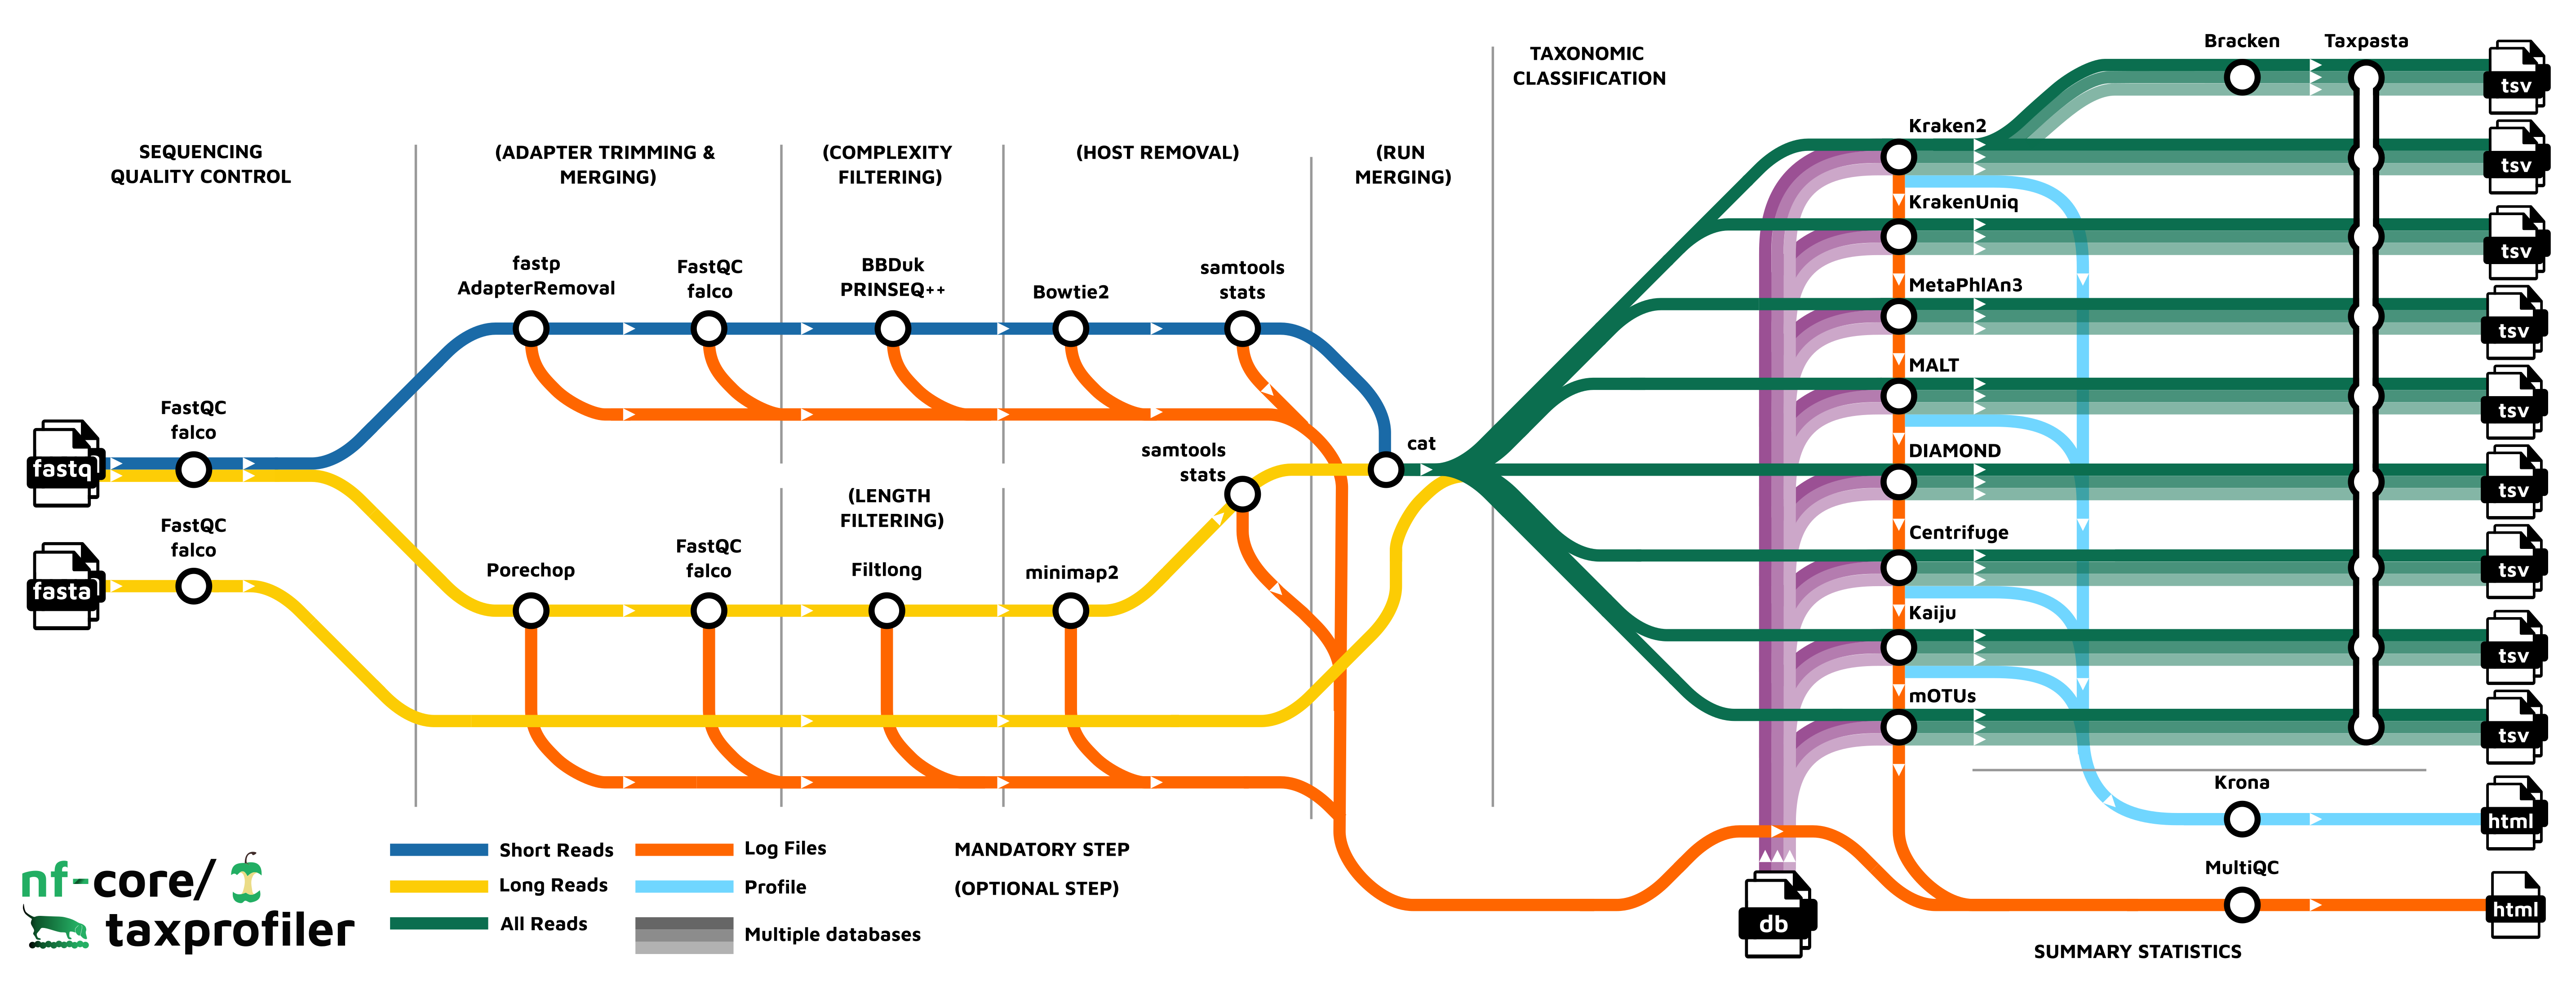
\includegraphics{taxprofiler_tube.png}

}

\caption{\label{fig-workflow-diagram}Visual overview of the
nf-core/taxprofiler workflow. nf-core/taxprofiler can take in FASTQ
(short or long reads) or FASTA files (long reads), that will optionally
go through sequencing quality control (e.g.~with FastQC), read
preprocessing (e.g.~removal of adapters), complexity filtering, host
removal, and run merging before performing taxonomic classification
and/or profiling with a user-selected range of tools and databases.
Output from all classifiers and profilers are standardised into a common
taxon table format, and when supported visualisations of the profiles
are generated.}

\end{figure}

\hypertarget{tbl-tool-summaries}{}
\begin{longtable}[]{@{}
  >{\raggedright\arraybackslash}p{(\columnwidth - 8\tabcolsep) * \real{0.1446}}
  >{\raggedright\arraybackslash}p{(\columnwidth - 8\tabcolsep) * \real{0.2289}}
  >{\raggedright\arraybackslash}p{(\columnwidth - 8\tabcolsep) * \real{0.1928}}
  >{\raggedright\arraybackslash}p{(\columnwidth - 8\tabcolsep) * \real{0.1446}}
  >{\raggedright\arraybackslash}p{(\columnwidth - 8\tabcolsep) * \real{0.2892}}@{}}
\caption{\label{tbl-tool-summaries}List of nf-core/taxprofiler supported
taxonomic/classifiers profilers as of version 1.1 and their approximate
method and supported input database types. Sequencing matching type
refers to which `molecular alphabet' is primarily used for matching
between a query (read) and a reference (genome/gene). Primary algorithm
refers to the algorithm type used for sequencing matching. Reference
type refers to the typical sequence type used in database construction
of the tool. Method refers to whether the tool performs just read
classification (classifier) or additionally abundance estimation
(profiler)}\tabularnewline
\toprule\noalign{}
\begin{minipage}[b]{\linewidth}\raggedright
Tool
\end{minipage} & \begin{minipage}[b]{\linewidth}\raggedright
Primary Algorithm
\end{minipage} & \begin{minipage}[b]{\linewidth}\raggedright
Reference Type
\end{minipage} & \begin{minipage}[b]{\linewidth}\raggedright
Method
\end{minipage} & \begin{minipage}[b]{\linewidth}\raggedright
Sequence Matching Type
\end{minipage} \\
\midrule\noalign{}
\endfirsthead
\toprule\noalign{}
\begin{minipage}[b]{\linewidth}\raggedright
Tool
\end{minipage} & \begin{minipage}[b]{\linewidth}\raggedright
Primary Algorithm
\end{minipage} & \begin{minipage}[b]{\linewidth}\raggedright
Reference Type
\end{minipage} & \begin{minipage}[b]{\linewidth}\raggedright
Method
\end{minipage} & \begin{minipage}[b]{\linewidth}\raggedright
Sequence Matching Type
\end{minipage} \\
\midrule\noalign{}
\endhead
\bottomrule\noalign{}
\endlastfoot
Kraken2 & k-mer based & whole-genome & classifier & Nucleotide \\
Kaiju & k-mer based & whole-genome & classifier & Amino Acid \\
Bracken & k-mer based & whole-genome & profiler & Nucleotide \\
KrakenUniq & k-mer based & whole-genome & profiler & Nucleotide \\
ganon & k-mer based & whole-genome & profiler & Nucleotide \\
KMCP & k-mer based & whole-genome & profiler & Nucleotide \\
MALT & alignment based & whole-genome & classifier & Nucleotide/Amino
Acid \\
DIAMOND & alignment based & whole-genome & classifier & Amino Acid \\
Centrifuge & alignment based & whole-genome & profiler & Nucleotide \\
MetaPhlAn & alignment based & marker-gene & profiler & Nucleotide \\
mOTUS & alignment based & marker-gene & profiler & Nucleotide \\
\end{longtable}

\hypertarget{discussion}{%
\section{Discussion}\label{discussion}}

A range of pipelines already exists for taxonomic profiling, however,
each have their own particular purpose and capabilities. We compared the
functionality of nf-core/taxprofiler against four other recently
published or released pipelines, selected based on their similarity of
purpose to nf-core/taxprofiler. The selection criteria and a more
detailed comparison between the five pipelines can be seen in the
\protect\hyperlink{supplementary-information}{Supplementary
Information}, however overall, while there was a general similarity
across all pipelines, nf-core/taxprofiler showed the greatest
accessibility and user choice, through the use of an established
workflow manager (Nextflow supporting 7 software environment/container
systems), supporting both CLI and GUI execution, and the number of
supported classifiers. Furthermore, it is unique in that is the only
pipeline to support supplying multiple database for all of the tools in
a single pipeline run.

\hypertarget{tbl-pipeline-comparison}{}
\begin{longtable}[]{@{}
  >{\raggedright\arraybackslash}p{(\columnwidth - 12\tabcolsep) * \real{0.0982}}
  >{\raggedright\arraybackslash}p{(\columnwidth - 12\tabcolsep) * \real{0.2109}}
  >{\raggedright\arraybackslash}p{(\columnwidth - 12\tabcolsep) * \real{0.1345}}
  >{\raggedright\arraybackslash}p{(\columnwidth - 12\tabcolsep) * \real{0.1491}}
  >{\raggedright\arraybackslash}p{(\columnwidth - 12\tabcolsep) * \real{0.1382}}
  >{\raggedright\arraybackslash}p{(\columnwidth - 12\tabcolsep) * \real{0.1200}}
  >{\raggedright\arraybackslash}p{(\columnwidth - 12\tabcolsep) * \real{0.1491}}@{}}
\caption{\label{tbl-pipeline-comparison}Comparison of functionality with
four recent taxonomic pipelines with similar functionality. A more
detailed textual comaprison can be found in the
\protect\hyperlink{supplementary-information}{Supplementary
Information}.}\tabularnewline
\toprule\noalign{}
\begin{minipage}[b]{\linewidth}\raggedright
Category
\end{minipage} & \begin{minipage}[b]{\linewidth}\raggedright
Criterion
\end{minipage} & \begin{minipage}[b]{\linewidth}\raggedright
StaG-mwc
\end{minipage} & \begin{minipage}[b]{\linewidth}\raggedright
sunbeam
\end{minipage} & \begin{minipage}[b]{\linewidth}\raggedright
Unipro UGENE
\end{minipage} & \begin{minipage}[b]{\linewidth}\raggedright
tama
\end{minipage} & \begin{minipage}[b]{\linewidth}\raggedright
nf-core/taxprofiler
\end{minipage} \\
\midrule\noalign{}
\endfirsthead
\toprule\noalign{}
\begin{minipage}[b]{\linewidth}\raggedright
Category
\end{minipage} & \begin{minipage}[b]{\linewidth}\raggedright
Criterion
\end{minipage} & \begin{minipage}[b]{\linewidth}\raggedright
StaG-mwc
\end{minipage} & \begin{minipage}[b]{\linewidth}\raggedright
sunbeam
\end{minipage} & \begin{minipage}[b]{\linewidth}\raggedright
Unipro UGENE
\end{minipage} & \begin{minipage}[b]{\linewidth}\raggedright
tama
\end{minipage} & \begin{minipage}[b]{\linewidth}\raggedright
nf-core/taxprofiler
\end{minipage} \\
\midrule\noalign{}
\endhead
\bottomrule\noalign{}
\endlastfoot
Information & Source code URL &
\url{https://github.com/ctmrbio/stag-mwc} &
\url{https://github.com/sunbeam-labs/sunbeam} &
\url{https://github.com/ugeneunipro/ugene} &
\url{https://github.com/jkimlab/TAMA} &
\url{https://github.com/nf-core/taxprofiler/} \\
Information & Evaluated version & 0.7.0 & 4 & 48 & githash: 3a22c8f &
1.1.0 \\
Information & Last release date & 2023-06-13 & 2023-08-08 & 2023-08-08 &
2022-03-02 & 2023-09-19 \\
Information & Publication year & Unpublished & 2019 & 2019 & 2020 & This
publication \\
Information & Publication DOI & Unpublished &
\href{https://doi.org/10.1186/s40168-019-0658-x}{10.1186/s40168-019-0658-x}
&
\href{https://doi.org/10.1093/bioinformatics/bty901}{10.1093/bioinformatics/bty901}
&
\href{https://doi.org/10.1186/s12859-020-3533-7}{10.1186/s12859-020-3533-7}
& This publication \\
Reproducibility & Pipeline versioning & Yes & Yes & Yes & No & Yes \\
Reproducibility & Software versioning & Yes & Yes & Yes & Yes & Yes \\
Reproducibility & Nr. software environments or container engines
supported & 2 & 2 & 0 & 1 & 7 \\
Accessibility & Installation documentation & Yes & Yes & Yes & Yes &
Yes \\
Accessibility & Usage documentation & Yes & Yes & Yes & Yes & Yes \\
Accessibility & Output documentation & Yes & Yes & Yes & Yes & Yes \\
Accessibility & CLI execution interface & Yes & Yes & No & Yes & Yes \\
Accessibility & GUI execution interface & No & No & Yes & No & Yes \\
Accessibility/Scalability & Integration a scheduling systems & Yes & Yes
& No & No & Yes \\
Portability/Accessibility & Nr. supported operating systems & 2 & 1 & 3
& 1 & 2 \\
Portability & Local machine integration & Yes & Yes & Yes & Yes & Yes \\
Portability/Scalability & HPC scheduler integration & Yes & Yes & No &
No & Yes \\
Portability/Scalability & Cloud computing integration & Unsure & Unsure
& No & No & Yes \\
Portability/Scalability & Integration with multiple scheduling systems &
Partial & Partial & No & No & Yes \\
Scalability & Per-process resource optimisation & Yes & Yes & Yes & No &
Yes \\
Functionality & Short read support & Yes & Yes & Yes & Yes & Yes \\
Functionality & Long read support & No & No & Yes & No & Yes \\
Functionality & Read preprocessing & Yes & Yes & Yes & Yes & Yes \\
Functionality & Sequencing depth estimation & Yes & No & No & No & No \\
Functionality & Complexity filtering & No & Yes & No & No & Yes \\
Functionality & Host removal & Yes & Yes & Partial & No & Yes \\
Functionality & Nr. supported taxonomic classifiers/profilers & 7 & 3 &
3 & 3 & 11 \\
Functionality & Graphical run reports & Yes & No & No & No & Yes \\
Functionality & Standardised profiles & No & No & No & Yes & Yes \\
Functionality & Multiple database supported & Partial & No & No & No &
Yes \\
Functionality & Metagenomic assembly & No & Yes & No & No & No \\
Functionality & Visualisation & No & No & No & No & Partial \\
\end{longtable}

An important advantage of nf-core/taxprofiler is that it is being
developed within the nf-core community (\url{https://nf-co.re}), that
provides strong long-term support for the continued community-based
development and maintenance of its pipelines. In this framework, we will
continue to add additional preprocessing, metagenomic classification,
and profiling tools as they become established and as requested by the
metagenomics community, for example, we feel that the inclusion of steps
such as sequencing saturation estimation as already being performed by
StaG-mwc would be beneficial to the nf-core/taxprofiler workflow
(possibly with dedicated tools such as Nonpareil (Rodriguez-R et al.
2018)), and/or more performant complexity filtering tools such as
Komplexity as offered by sunbeam. This also applies to extend support to
other sequencing platforms; nf-core/taxprofiler already supports
Nanopore long-read data, however the use of long-read PacBio data for
metagenomic data is growing in interest (Portik, Brown, and Pierce-Ward
2022). We are therefore considering adding dedicated preprocessing steps
for this type of sequencing data.

A remaining major challenge for metagenomics researchers (and not
supported in the same workflow by any of the compared pipelines above)
is the construction of databases for each profiling tool. Given there
still are no curated, high-quality `gold standard' databases in
metagenomics, and while nf-core/taxprofiler allows the profiling against
multiple databases and settings in parallel, currently the pipeline
still requires users to construct these manually and to supply to the
pipeline. While we feel this is currently a reasonable investment as
such databases can be repeatedly re-used, we are exploring the
possibility to add an additional complementary workflow in the pipeline
to allow automated database construction of all classification tools,
given a set of FASTA reference files.

Finally, once an overall taxonomic profile is generated, researchers
often wish to validate hits through more sensitive and accurate methods
such as with read-mapping alignment. While read alignment is supported
by other pipelines such as StaG-mwc, this happens in-parallel to the
taxonomic profiling and requires prior expectation of which reference
genomes to map against. Instead, nf-core/taxprofiler could be easily
extended to have a validation step similar to that of the ancient DNA
metagenomic pipeline aMeta (Pochon et al. 2022) where, utilising
Nextflow's execution parallelism, the input sequences could be aligned
back to the reference genomes of only those species with hits from the
taxonomic classification with dedicated accurate short- or long-read
aligners. In addition to the more precise classification,
post-classification read-alignment could also be particularly useful for
researchers in palaeogenomics who wish to use tools other than
KrakenUniq for initial classification (as in aMeta), where alignment
information can be used to authenticate ancient DNA within their samples
but also in clinical metagenomics to identify potential pathogens at
much finer resolution (e.g.~down to strain level).

Another motivation for developing nf-core/taxprofiler, despite the large
number of existing metagenomics pipelines is that by establishing a
taxonomic profiling pipeline within the nf-core ecosystem, it is
possible to begin building both standalone but also an integrated suite
of powerful interconnected pipelines for the major stages of metagenomic
workflows. Existing microbial- and metagenomics- related pipelines
within the nf-core initiative include nf-core/ampliseq (Straub et al.
2020), nf-core/mag (Krakau et al. 2022), and nf-core/funcscan
(\url{https://nf-co.re/funcscan}). We expect over time the ability to
link inputs and outputs of each workflow to develop comprehensive
metagenomic analyses, while still maintaining powerful standalone
pipelines, providing maximal user choice.

\hypertarget{conclusion}{%
\section{Conclusion}\label{conclusion}}

nf-core/taxprofiler is an accessible, efficient, and scalable pipeline
for metagenomic taxonomic classification and profiling that can be
executed on anywhere from laptops to the cloud. Offering, to our
knowledge, the largest number of taxonomic profilers across similar
pipelines, it provides flexibility for users not just on choice of
profiling tool but also with databases and database settings, with any
number being able to be supplied to the pipeline in a single run. We
hope that through detailed documentation and a range of execution
options, nf-core/taxprofiler will make reproducible and high-throughput
metagenomics more accessible for a wide range of disciplines.

\hypertarget{data-availability}{%
\section{Data Availability}\label{data-availability}}

All data used in this publication

\hypertarget{code-availability}{%
\section{Code Availability}\label{code-availability}}

nf-core/taxprofiler source code is available on GitHub at
\url{https://github.com/nf-core/taxprofiler}, and each release is
archived on Zenodo (latest version DOI:
\href{https://doi.org/10.5281/zenodo.7728364}{10.5281/zenodo.7728364})

The version of the pipeline described in this paper is version (1.1.0)
(release specific Zenodo archive DOI:
\href{https://doi.org/10.5281/zenodo.8358147}{10.5281/zenodo.8358147})

\hypertarget{supplementary-data}{%
\section{Supplementary Data}\label{supplementary-data}}

\hypertarget{acknowledgments}{%
\section{Acknowledgments}\label{acknowledgments}}

We thank Prof.~Christina Warinner and the Microbiome Sciences group
MPI-EVA for original discussions that lead to the pipeline. We are also
grateful for the nf-core community for the original and ongoing support
in the development in the pipeline, in particular for the contributions
by Lauri Mesilaakso, Jianhong Ou, and Rafał Stępień.

\hypertarget{funding}{%
\section{Funding}\label{funding}}

S.S. and L.A-L. were supported by Rapid establishment of comprehensive
laboratory pandemic preparedness -- RAPID-SEQ. This material is based
upon work supported by the U.S. Department of Agriculture, Agricultural
Research Service, under agreement No.~58-3022-0-001 (T.A.C II). M.B. and
J.A.F.Y were supported by the Max Planck Society. J.A.F.Y was supported
by the Werner Siemens-Stiftung (``Paleobiotechnology'', Awarded to
Prof.~Pierre Stallforth and Prof.~Christina Warinner).

\hypertarget{supplementary-information}{%
\section{Supplementary Information}\label{supplementary-information}}

\hypertarget{implementation}{%
\subsection{Implementation}\label{implementation}}

\hypertarget{input-and-execution}{%
\subsubsection{Input and Execution}\label{input-and-execution}}

The pipeline can be executed via typical Nextflow commands, or using the
standard nf-core `launch' GUI
(\url{https://nf-co.re/taxprofiler/launch}), making the pipeline
accessible for both computationally experienced as well as less
experienced researchers. In addition to the general usage and parameter
documentation of the pipeline (https://nf-co.re/taxprofiler). The GUI
offers immediate assistance and guidance to users on what each parameter
does, both in short- and long-form, with long-form parameter
descriptions additionally describing which tool-specific parameters are
being modified for each pipeline parameter
(Figure~\ref{fig-launch-page}). The GUI also includes controlled user
input by providing strict drop-down lists and input validation prior
execution of the pipeline to reduce the risk of typos and other mistakes
(in contrast to the command-line interface (CLI) that only includes
validation at pipeline run-time).

\begin{figure}

{\centering 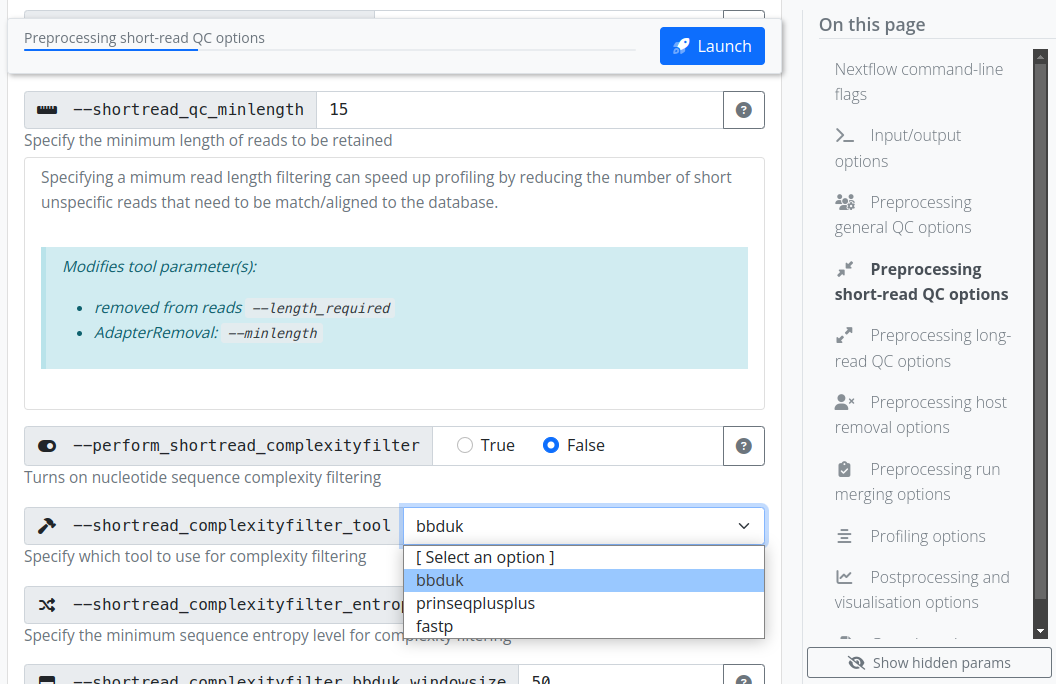
\includegraphics{taxprofiler_launchpage.png}

}

\caption{\label{fig-launch-page}Screenshot of the nf-core pipeline
launch graphical user interface with nf-core/taxprofiler options
displayed. The web browser-based interface provides guidance for how to
configure each pipeline parameter by providing both short and long help
descriptions to help guide users in which contexts to configure each
parameter. Additional elements such as radio buttons, drop down menus,
and background regular expressions check for validity of input. When
pressing launch, a prepared configuration file and command is provided
that can be copied and pasted by the user into the terminal}

\end{figure}

An example nf-core command line execution of the pipeline can be seen in
Code Block~\ref{lst-example-cmd}, where two input files are supplied:
one file specifying paths of FASTQ files of metagenomic samples and
necessary metadata for preprocessing (such as sample ID and sequencing
platform), and the second file specifying paths to the user-defined
databases with per-database classification parameters. Various
parameters are available to select different preprocessing steps, and
provide additional configuration such as tool selection and value
options. Note that even if a user supplies a given database in the
database input sheet, the corresponding profiling tool must still be
activated with the corresponding pipeline parameter
(e.g.~\texttt{-\/-run\_kraken2}). Per-classifier flags are also
available for the optional saving of additional non-profile output
files.

\begin{codelisting}

\caption{Example nf-core/taxprofiler command for running short-read
quality control, removal of host DNA and executing the k-mer based
Kraken2 and marker gene alignment MetaPhlAn3 tools.}

\hypertarget{lst-example-cmd}{%
\label{lst-example-cmd}}%
\begin{Shaded}
\begin{Highlighting}[]
\ExtensionTok{$}\NormalTok{ nextflow run nf{-}core/taxprofiler }\DataTypeTok{\textbackslash{}}
    \AttributeTok{{-}r}\NormalTok{ 1.1.0 }\DataTypeTok{\textbackslash{}}
    \AttributeTok{{-}profile}\NormalTok{ singularity,}\OperatorTok{\textless{}}\NormalTok{institute}\OperatorTok{\textgreater{}} \DataTypeTok{\textbackslash{}}
    \AttributeTok{{-}{-}input} \OperatorTok{\textless{}}\NormalTok{samplesheet.csv}\OperatorTok{\textgreater{}} \DataTypeTok{\textbackslash{}}
    \AttributeTok{{-}{-}databases} \OperatorTok{\textless{}}\NormalTok{database.csv}\OperatorTok{\textgreater{}} \DataTypeTok{\textbackslash{}}
    \AttributeTok{{-}{-}perform\_shortread\_qc} \DataTypeTok{\textbackslash{}}
    \AttributeTok{{-}{-}shortread\_qc\_minlength}\NormalTok{ 20 }\DataTypeTok{\textbackslash{}}
    \AttributeTok{{-}{-}preprocessing\_qc\_tool}\NormalTok{ falco }\DataTypeTok{\textbackslash{}}
    \AttributeTok{{-}{-}run\_host\_removal} \AttributeTok{{-}{-}hostremoval\_reference} \StringTok{\textquotesingle{}host\_genome.fasta\textquotesingle{}} \DataTypeTok{\textbackslash{}}
    \AttributeTok{{-}{-}run\_kraken2} \AttributeTok{{-}{-}kraken2\_save\_reads} \DataTypeTok{\textbackslash{}}
    \AttributeTok{{-}{-}run\_metaphlan3} \DataTypeTok{\textbackslash{}}
    \AttributeTok{{-}{-}run\_krona} \DataTypeTok{\textbackslash{}}
    \AttributeTok{{-}{-}run\_profile\_standardisation}
\end{Highlighting}
\end{Shaded}

\end{codelisting}

All nf-core pipelines are strictly versioned (specified with the
Nextflow \texttt{-r} flag), and to ensure reproducibility, each version
of the pipeline has a fixed set of software used for each step of the
pipeline. The fixed set of software are controlled through the use of
the conda package manager or containers (e.g., Docker, or Apptainer
-previously known as Singularity) from the stable Bioconda (Grüning et
al. 2018) or BioContainers (Veiga Leprevost et al. 2017) repositories.
This, coupled with the intrinsic Nextflow ability to execute on most
infrastructure whether that is a local laptop (resource requirements
permitting), traditional HPC, as well across common cloud providers also
makes nf-core/taxprofiler a very portable pipeline that can be used in
many contexts.

\hypertarget{preprocessing}{%
\subsubsection{Preprocessing}\label{preprocessing}}

Preprocessing steps in nf-core/taxprofiler are aimed at removing
laboratory and sequencing artefacts that may influence taxonomic
profiling, either for computing resource consumption or and/or
false-positive or false-negative classification reasons. First
sequencing quality control with FastQC (Andrews 2010) or Falco (Sena
Brandine and Smith 2021) is carried out. Falco was included for reduced
memory requirements, in particular for long read sequencing data.
Artificial library adapter sequences added during sequencing reduce
sequencing matching accuracy by reducing sequence specificity, and in
some cases, may result in false-positive hits due to adapter sequence
contamination in reference genomes (Schäffer et al. 2018; F. P.
Breitwieser, Baker, and Salzberg 2018) \footnote{For an `infamous' case
  of adapter sequences in a published eukaryotic genome, see the
  following blog posts

  Graham Etherington:
  \url{https://web.archive.org/web/20201219022000/http://grahametherington.blogspot.com/2014/09/why-you-should-qc-your-reads-and-your.html?m=1}why-you-should-qc-your-reads-and-your.html
  Sixing Huang:
  \url{https://web.archive.org/web/20220904205331/https://dgg32.medium.com/carp-in-the-soil-1168818d2191}

  (Accessed 2023-08-25)}. Additionally, paired-end merging may provide
longer sequences that will allow for more specific classification when
paired-end alignment is not supported by a given classifier. For these
tasks nf-core/taxprofiler can apply either fastp (Chen et al. 2018) or
AdapterRemoval2 (Schubert, Lindgreen, and Orlando 2016) for short reads,
and currently Porechop (Wick et al. 2017) for Oxford Nanopore long-read
data. For both short and long reads, FastQC or Falco is run again to
allow assessment on the performance of the adapter removal and/or
pair-merging step.

Low complexity sequences, e.g.~sequences containing long stretches of
mono- or di-nucleotide repeats provide little specific genetic
information that contribute to taxonomic identification, as they can
align to many different reference genomes (Schmieder and Edwards 2011;
Clarke et al. 2019). Including such reads during taxonomic profiling can
increase run-time and memory usage for little gain, as during
lowest-common-ancestor (LCA) classification steps they will be assigned
to high-level taxonomic ranks (e.g.~Kingdom). nf-core/taxprofiler
performs removal of these reads through complexity filtering algorithms
as provided by fastp, BBDuk (Bushnell 2022), or PRINSEQ++ (Cantu,
Sadural, and Edwards 2019). Long read sequences often do not have such
reads, as lengths are sufficient enough to capture greater sequence
diversity - but it is sometimes desirable to only classify reads longer
than a certain length - as these provide more precise taxonomic
information (Dilthey et al. 2019; Portik, Brown, and Pierce-Ward 2022).
Therefore, nf-core/taxprofiler can remove reads shorter than a
user-defined length using Filtlong.

Removing host DNA is another common preprocessing step in metagenomic
studies. This can help speed up run-time, particularly in microbiome
studies, where detection of microbes are of interest. Furthermore,
host-contamination of reference genomes in public databases is common
(Longo, O'Neill, and O'Neill 2011; Kryukov and Imanishi 2016; Florian P.
Breitwieser et al. 2019) and therefore the removal of such sequences can
also decrease the risk of false positive taxonomic assignment. To remove
multiple hosts or other sequences, all reference genomes can be combined
into a single FASTA reference file. Short read host removal can be
carried out with Bowtie2 (Langmead and Salzberg 2012; Langmead et al.
2019) and minimap2 (Li 2018) for long reads, both in combination with
SAMtools (Li et al. 2009; Danecek et al. 2021), where reads are aligned
against the reference genome and the off-target (unaligned) reads are
then converted back to FASTQ format for classification.

Finally, nf-core/taxprofiler can optionally perform run merging where
libraries have been sequenced over multiple lanes to generate one
profile per sample or library. The final set of reads used for profiling
can be optionally saved for downstream re-use. Throughout all steps,
relevant statistics and log files are generated and used both for the
final pipeline run report as well as saved into the results directory of
the pipeline run for further inspection where necessary.

\hypertarget{profiling}{%
\subsubsection{Profiling}\label{profiling}}

There are many types of metagenomic profiling techniques, from profiling
against whole-genome references with alignment or k-mer based
approaches, to methods involving alignment to species-specific
marker-gene families (Quince et al. 2017; Ye et al. 2019).
nf-core/taxprofiler aims to support and include all established
classification or profiling tools as requested by the community. The
choice of tools used in a pipeline run is up to the user, with a tool
being executed when both the corresponding database and
\texttt{-\/-run\_\textless{}tool\textgreater{}} flag is provided.
Specific classification settings for each tool and database are
specified in the database CSV input sheet. Some tools also have pipeline
level command-line flags for controlling certain aspects of output
files.

As of version 1.1.0, the following classifiers and profilers are
available: Kraken2 (Wood, Lu, and Langmead 2019), Bracken (Lu et al.
2017), KrakenUniq (F. P. Breitwieser, Baker, and Salzberg 2018),
Centrifuge (Kim et al. 2016), MALT (Vågene et al. 2018), DIAMOND
(Buchfink, Reuter, and Drost 2021), Kaiju (Menzel, Ng, and Krogh 2016),
MetaPhlAn (Blanco-Míguez et al. 2023), mOTUs (Ruscheweyh et al. 2022),
ganon (Piro et al. 2020), KMCP (Shen et al. 2023).
Table~\ref{tbl-tool-summaries} summarises the category and reference
database type for each tool.

By default, nf-core/taxprofiler produces the per-sample main taxonomic
classification profile from a tool or a tool's report generation tool.
The output is normally in the form of counts per reference sequencing,
with additional statistics about the hits of a particular organism
(estimated abundance, taxonomic level etc.). Users can also optionally
request output of per-read classification output, and output such as
classified and unclassified reads in FASTQ format, where supported.

The pipeline provides high efficiency, particularly during the
metagenomic classification stage, through the inherent parallelisation
provided by Nextflow. While metagenomic classification is comparatively
computationally intensive (in terms of memory and execution time; due to
a combination of sequencing depth and number of reference genomes),
Nextflow automatically optimises the execution order of all the steps in
pipeline, maximising the number parallel running of multiple profilers
and/or databases at any given time point, as far as the available
computational resources allow. For local machines such as laptops or
desktops, Nextflow will automatically detect all available computational
resources but this is customisable using Nextflow configuration files.
For HPC and cloud infrastructure, users typically have to define the
computational infrastructural environment the pipeline is being executed
on (CPU or memory limitations, queues, instance types, etc.). To
facilitate the pipeline set-up, nf-core/taxprofiler supports pre-defined
centralised generic and pipeline-specific institutional Nextflow
configurations as provided by nf-core/configs
(\url{https://nf-co.re/configs}; more than 90 institutions at the time
of writing). However, users are still welcome to supply their own custom
configuration files, further refining computational limitations or
execution specifications.

\hypertarget{post-profiling}{%
\subsubsection{Post-profiling}\label{post-profiling}}

In metagenomic studies, it is common practise to compare the profiles
among many samples, and the results of multiple profiles are normally
stored in `taxon tables', i.e, counts per reference taxon (rows), for
each sample (columns). When available, nf-core/taxprofiler supports the
option to produce the `native' taxon table of each classification tool
when multiple samples are run.

One of the challenges that researchers face when comparing multiple
taxonomic classifiers or profilers is the heterogenous output formats
that are produced, that often require custom parsing and merging scripts
for each tool to standardise. To facilitate more user-friendly
cross-comparisons between tools, nf-core/taxprofiler utilises the
TAXPASTA tool (Beber et al. 2023) to generate standardised profiles and
generate multi-sample tables.

Summary statistics for the entire pipeline are visualised and displayed
in a customisable MultiQC report (Ewels et al. 2020). When supported,
quality control of data and pipeline runs are shown for manual
verification. Krona plots (Ondov, Bergman, and Phillippy 2011) can also
optionally be generated for supported tools to help provide further
visualisation of taxonomic profiles.

\hypertarget{output}{%
\subsubsection{Output}\label{output}}

To summarise, the main default output from nf-core/taxprofiler are both
classifier `native' and standardised single- and multi-sample taxonomic
profiles with counts per-taxon and an interactive MultiQC run report
with all run statistics, in addition to the raw log files themselves
where available.

The MultiQC run report displays statistics and summary visualisations
for all steps of the pipeline where possible, lists of versions for all
tools of each step of the pipeline, and provides a
dynamically-constructed text for the recommended `methods' text for
reporting how the pipeline was executed (including relevant citations)
that users can use in their own publications.

Optional outputs can include other types of profiles (e.g.~per read
classification) and in other formats as produced by the tools
themselves, as well as raw reads from preprocessing steps and output
visualisations from Krona. Nextflow resource usage and trace reports are
also by default produced for users to check pipeline performance.

\hypertarget{comparison-with-other-solutions}{%
\subsection{Comparison with other
solutions}\label{comparison-with-other-solutions}}

nf-core/taxprofiler has been specifically developed for the analysis of
whole-genome, \emph{metagenomic} sequencing data. While other types of
taxonomic profiling data such as 16S amplicon sequencing are well
established fields with a range of popular high-quality and
best-practise tools pipelines (e.g. (Blanco-Míguez et al. 2023; Schloss
et al. 2009)) and databases (DeSantis et al. 2006; Yilmaz et al. 2014),
`gold standard' tools and databases for metagenomics remain much less
established. Thus, the need for highly-multiplexed classification is
more desirable for the newer metagenomics methods. Despite this, tools
such as METAXA2 (Bengtsson-Palme et al. 2015) that use shotgun
sequencing reads to recover 16S sequences from metagenomic samples.

We searched Google Scholar for open-source pipelines published or
released in the last 5 years (at the time of writing, since 2018) that
were designed primarily for metagenomic classification screening, that
supported at least 2 classifiers, had at least one preprocessing step
and were not specifically targeted at read classification of specific
domains of taxa (e.g.~viruses or bacteriophages only). We also included
an additional pipeline at the recommendations of the authors of the
pipeline due to the functional overlap to nf-core/taxprofiler. We then
evaluated the pipelines based on their publications and documentation
for typical metagenomic profiling workflow steps, and a range of
criteria related to expectations of modern bioinformatic workflows that
can be summarised in the following four criteria: reproducibility,
accessibility, scalability, and portability (Wratten, Wilm, and Göke
2021). After searching, we selected the following pipelines for
comparison with nf-core/taxprofiler: sunbeam (v4, Clarke et al. 2019),
Unipro UGENE (v48, Rose et al. 2019), TAMA (githash: 3a22c8f, Sim et al.
2020), and StaG-mwc (0.7.0, Boulund et al. 2023).

In terms of accessibility, all pipelines have documentation describing
the installation steps, usage instructions, and output files. However,
there are varying levels of detail and comprehensiveness. In particular,
StaG-mwc and nf-core/taxprofiler have the most detailed descriptions of
all possible output files for every supported module, whereas Unipro
UGENE and sunbeam have very minimal to possibly unfinished output
documentation. For execution options, most of the pipelines provide CLI
execution, except for Unipro UGENE which offers only GUI-based pipeline
set-up (despite a command-line execution of the GUI generated
configuration). In particular, nf-core/taxprofiler is the only pipeline
providing both CLI and GUI interfaces for pipeline run execution.

Criteria covering portability also overlap with accessibility, as it
implies options for and ease of different users running on different
types of computing infrastructure, whether that is on their own laptop,
on an HPC cluster, or in the cloud. Unipro UGENE is the only pipeline
that supports execution on all three major operating systems (Linux,
OSX, Windows), whereas StaG-mwc and nf-core/taxprofiler can be run on
unix operating systems, and sunbeam and TAMA are only being supported on
Linux. While all pipelines support `local' machine execution
(e.g.~personal laptops or desktops), a large portion of academic users
execute computationally intensive bioinformatic tasks on HPC clusters.
In these contexts, pipeline task submissions are normally managed by job
schedulers, thus integration with schedulers is an important criterion
for running large multi-step and parallelised pipelines. The three
pipelines leveraging workflow managers (Snakemake (Mölder et al. 2021)
and Nextflow) support integration with schedulers (StaG-mwc, sunbeam,
and nf-core/taxprofiler) with nf-core/taxprofiler supporting the most by
far
(\href{https://www.nextflow.io/docs/latest/executor.html}{\textgreater10
scheduling systems}) as natively offered by Nextflow. This allows the
greatest possible choice for users in terms of which HPC infrastructure
they can execute their pipeline on. As an extension of this, only
nf-core/taxprofiler has explicit support for cloud computing (e.g.~AWS,
GCP, or Microsoft Azure), again maximising user choice and portability
when it comes to running the pipeline.

In terms of scalability, the aforementioned integration with schedulers
and cloud computing support implicitly maximises efficiency and
parallellisation of pipeline runs, providing good scalability for
varying numbers of input files and steps in the pipeline. Again, the
three workflow manager based pipelines provide scalability, whereas
there is no mention neither Unipro UGENE nor TAMA in reference to
parallel task execution. Furthemore, all pipelines except TAMA, allowed
per-process customisation of computational resources, something critical
for maximising efficient scalability to ensure only the necessary
resources for a given step of a pipeline are requested.

In terms of reproducibility, all five pipelines are good at ensuring
reproducibility in terms of pipeline and software versioning (allowing
re-execution of pipeline runs using the same software), with only tama
not having stable versioned releases. However, installing software
manually across different infrastructures can result in variability in
the execution of each software \footnote{As demonstrated in this
  blogpost from Paweł Przytuła:
  \url{https://web.archive.org/web/20230320223436/https://appsilon.com/reproducible-research-when-your-results-cant-be-reproduced/}
  (Accessed 2023-08-25)} (Di Tommaso et al. 2017).The current most
popular solution to the problem of inconsistent software environments is
to use container engines such as Docker or Apptainer to run container
images which are isolated, deterministic computing environments which
can be executed by any system providing a container runtime. Only Unipro
UGENE does not document the use of a container system, with
nf-core/taxprofiler offering the biggest choice for users courtesy of
Nextflow (6 different engine systems at the time of writing).

Finally, we compared metagenomics related functionality between the
pipelines. All pipelines support short-read FASTQ input, but only
nf-core/taxprofiler explicitly reports long-read support, while the
documentation in Unipro UGENE states that assembled contigs are possible
input to some of the profilers. All pipelines support read preprocessing
(adapter clipping, and merging). In terms of tools used for
preprocessing, Trimmomatic (Bolger, Lohse, and Usadel 2014) is popular
across the other pipelines but is not supported in nf-core/taxprofiler.
Only sunbeam and nf-core/taxprofiler support complexity filtering to
remove low sequence diversity reads. In fact within sunbeam, the authors
developed their own dedicated, performant complexity filtering tool
Komplexity (Clarke et al. 2019). Most pipelines support some form of
host removal (only TAMA did not support this), and it is likely possible
with Unipro UGENE through user customisation of the workflow. In all
cases, host removal consists of mapping processed reads with an aligner
and using the off-target reads for downstream profiling (as implemented
in nf-core/taxprofiler), however StaG-mwc has an additional separate
metagenomic host removal step with Kraken2. nf-core/taxprofiler supports
by far the largest number of taxonomic classifers and profilers at 11 as
of v1.1.0 - providing the greatest choice to users - with StaG-mwc
offering 7, and the remaining pipelines only 3. Only nf-core/taxprofiler
and partly StaG-mwc explicitly support running each profiler with
multiple databases. nf-core/taxprofiler is the only pipeline that
supports running an arbitrary number of different metagenomic profiler
databases each with their own settings - making it useful for tool
parameter comparison, testing different databases, or reducing the size
of each database (e.g.~per domain) to make it more flexibility for
running on smaller computational infrastructure. StaG-mwc allows
multiple references for their short-read alignment steps rather than the
metagenomic profilers. For output, nf-core/taxprofiler, StaG-mwc, and
sunbeam (via an extension) support a singular run report for summarising
all preprocessing step. Only nf-core/taxprofiler and TAMA produce
standardised output for all taxonomic profilers (via TAXPASTA). However
Unipro UGENE additionally offers a `consensus' profile using WEVOTE
(Metwally et al. 2016).

To summarise, many of the pipelines reviewed here offer similar
functionality, with particularly StaG-mwc having a strong overlap with
nf-core/taxprofiler. Thus, users in most cases will be able to select
the pipeline depending on which framework they feel most comfortable
with. However the advantages of nf-core/taxprofiler mainly come from the
offering of the greatest choice of tools, the benefits provided by
Nextflow whereby it provides the greatest number of computational
infrastructure types the pipeline can be executed on, and container
systems can be used to ensure reproducibility, and the support of the
nf-core community due to the centralised pool of `plug-and-play' modules
to make it easier to update the pipeline over time to add new tool.

The functionality offered by other pipelines not currently supported by
nf-core/taxprofiler include sequencing saturation estimation (StaG-mwc),
taxonomy-free composition comparison (StaG-mwc), functional profiling
(StaG-mwc) , \emph{de novo} assembly (sunbeam) , and reference mapping
(StaG-mwc, sunbeam). We do not plan to support \emph{de novo} assembly
or functional profiling in nf-core/taxprofiler as we feel this better
served by other existing dedicated pipelines (e.g. Uritskiy, DiRuggiero,
and Taylor 2018; Krakau et al. 2022).

We note there exists a range of other pipelines that also include some
form of taxonomic classification. However often these pipelines have
been developed with a different main purpose (e.g.~Assembly and binning
for nf-core/mag (Krakau et al. 2022), MetaWRAP (Uritskiy, DiRuggiero,
and Taylor 2018), SqueezeMeta (Tamames and Puente-Sánchez 2018), or
MEDUSA (Morais et al. 2022); Metagenomic read alignment with CCMetaGen
(Marcelino et al. 2020) and Wochenende (Rosenboom et al. 2022)).

\hypertarget{references}{%
\section*{References}\label{references}}
\addcontentsline{toc}{section}{References}

\hypertarget{refs}{}
\begin{CSLReferences}{1}{0}
\leavevmode\vadjust pre{\hypertarget{ref-Andrews2010-pd}{}}%
Andrews, Simon. 2010. {``{FastQC}: A Quality Control Tool for High
Throughput Sequence Data.''}
\url{http://www.bioinformatics.babraham.ac.uk/projects/fastqc/}.

\leavevmode\vadjust pre{\hypertarget{ref-Beber2023-hk}{}}%
Beber, Moritz E, Maxime Borry, Sofia Stamouli, and James A Fellows
Yates. 2023. {``{TAXPASTA}: {TAXonomic} Profile Aggregation and
{STAndardisation}.''} \emph{Journal of Open Source Software} 8 (87):
5627. \url{https://doi.org/10.21105/joss.05627}.

\leavevmode\vadjust pre{\hypertarget{ref-Bengtsson-Palme2015-ar}{}}%
Bengtsson-Palme, Johan, Martin Hartmann, Karl Martin Eriksson, Chandan
Pal, Kaisa Thorell, Dan Göran Joakim Larsson, and Rolf Henrik Nilsson.
2015. {``{METAXA2}: Improved Identification and Taxonomic Classification
of Small and Large Subunit {rRNA} in Metagenomic Data.''}
\emph{Molecular Ecology Resources} 15 (6): 1403--14.
\url{https://doi.org/10.1111/1755-0998.12399}.

\leavevmode\vadjust pre{\hypertarget{ref-Blanco-Miguez2023-cq}{}}%
Blanco-Míguez, Aitor, Francesco Beghini, Fabio Cumbo, Lauren J McIver,
Kelsey N Thompson, Moreno Zolfo, Paolo Manghi, et al. 2023. {``Extending
and Improving Metagenomic Taxonomic Profiling with Uncharacterized
Species Using {MetaPhlAn} 4.''} \emph{Nature Biotechnology}, February,
1--12. \url{https://doi.org/10.1038/s41587-023-01688-w}.

\leavevmode\vadjust pre{\hypertarget{ref-Bolger2014-pm}{}}%
Bolger, Anthony M, Marc Lohse, and Bjoern Usadel. 2014. {``Trimmomatic:
A Flexible Trimmer for Illumina Sequence Data.''} \emph{Bioinformatics
(Oxford, England)} 30 (15): 2114--20.
\url{https://doi.org/10.1093/bioinformatics/btu170}.

\leavevmode\vadjust pre{\hypertarget{ref-Boulund2023-ct}{}}%
Boulund, Fredrik, Aron Arzoomand, Justine Debelius, chrsb, and Lisa
Olsson. 2023. {``Ctmrbio/Stag-Mwc: {StaG} {v0}.7.0.''} Zenodo.
\url{https://doi.org/10.5281/ZENODO.8032462}.

\leavevmode\vadjust pre{\hypertarget{ref-Breitwieser2018-xg}{}}%
Breitwieser, F P, D N Baker, and S L Salzberg. 2018. {``{KrakenUniq}:
Confident and Fast Metagenomics Classification Using Unique k-Mer
Counts.''} \emph{Genome Biology} 19 (1): 198.
\url{https://doi.org/10.1186/s13059-018-1568-0}.

\leavevmode\vadjust pre{\hypertarget{ref-Breitwieser2019-ys}{}}%
Breitwieser, Florian P, Jennifer Lu, and Steven L Salzberg. 2019. {``A
Review of Methods and Databases for Metagenomic Classification and
Assembly.''} \emph{Briefings in Bioinformatics} 20 (4): 1125--36.
\url{https://doi.org/10.1093/bib/bbx120}.

\leavevmode\vadjust pre{\hypertarget{ref-Breitwieser2019-iz}{}}%
Breitwieser, Florian P, Mihaela Pertea, Aleksey Zimin, and Steven L
Salzberg. 2019. {``Human Contamination in Bacterial Genomes Has Created
Thousands of Spurious Proteins.''} \emph{Genome Research} 29 (May):
954--60. \url{https://doi.org/10.1101/gr.245373.118}.

\leavevmode\vadjust pre{\hypertarget{ref-Buchfink2021-ks}{}}%
Buchfink, Benjamin, Klaus Reuter, and Hajk-Georg Drost. 2021.
{``Sensitive Protein Alignments at Tree-of-Life Scale Using
{DIAMOND}.''} \emph{Nature Methods} 18 (4): 366--68.
\url{https://doi.org/10.1038/s41592-021-01101-x}.

\leavevmode\vadjust pre{\hypertarget{ref-Bushnell2022-pf}{}}%
Bushnell, Brian. 2022. {``{BBMap}.''}
\url{https://sourceforge.net/projects/bbmap/}.

\leavevmode\vadjust pre{\hypertarget{ref-Cantu2019-lh}{}}%
Cantu, Vito Adrian, Jeffrey Sadural, and Robert Edwards. 2019.
{``{PRINSEQ++}, a Multi-Threaded Tool for Fast and Efficient Quality
Control and Preprocessing of Sequencing Datasets.''} e27553v1. PeerJ
Preprints; PeerJ Inc.
\url{https://doi.org/10.7287/peerj.preprints.27553v1}.

\leavevmode\vadjust pre{\hypertarget{ref-Chen2018-vg}{}}%
Chen, Shifu, Yanqing Zhou, Yaru Chen, and Jia Gu. 2018. {``Fastp: An
Ultra-Fast All-in-One {FASTQ} Preprocessor.''} \emph{Bioinformatics} 34
(17): i884--90. \url{https://doi.org/10.1093/bioinformatics/bty560}.

\leavevmode\vadjust pre{\hypertarget{ref-Chiu2019-mv}{}}%
Chiu, Charles Y, and Steven A Miller. 2019. {``Clinical Metagenomics.''}
\emph{Nature Reviews. Genetics} 20 (6): 341--55.
\url{https://doi.org/10.1038/s41576-019-0113-7}.

\leavevmode\vadjust pre{\hypertarget{ref-Clarke2019-al}{}}%
Clarke, Erik L, Louis J Taylor, Chunyu Zhao, Andrew Connell, Jung-Jin
Lee, Bryton Fett, Frederic D Bushman, and Kyle Bittinger. 2019.
{``Sunbeam: An Extensible Pipeline for Analyzing Metagenomic Sequencing
Experiments.''} \emph{Microbiome} 7 (1): 46.
\url{https://doi.org/10.1186/s40168-019-0658-x}.

\leavevmode\vadjust pre{\hypertarget{ref-Danecek2021-gj}{}}%
Danecek, Petr, James K Bonfield, Jennifer Liddle, John Marshall, Valeriu
Ohan, Martin O Pollard, Andrew Whitwham, et al. 2021. {``Twelve Years of
{SAMtools} and {BCFtools}.''} \emph{GigaScience} 10 (2).
\url{https://doi.org/10.1093/gigascience/giab008}.

\leavevmode\vadjust pre{\hypertarget{ref-DeSantis2006-cm}{}}%
DeSantis, T Z, P Hugenholtz, N Larsen, M Rojas, E L Brodie, K Keller, T
Huber, D Dalevi, P Hu, and G L Andersen. 2006. {``Greengenes, a
Chimera-Checked {16S} {rRNA} Gene Database and Workbench Compatible with
{ARB}.''} \emph{Applied and Environmental Microbiology} 72 (7):
5069--72. \url{https://doi.org/10.1128/AEM.03006-05}.

\leavevmode\vadjust pre{\hypertarget{ref-Di_Tommaso2017-xu}{}}%
Di Tommaso, Paolo, Maria Chatzou, Evan W Floden, Pablo Prieto Barja,
Emilio Palumbo, and Cedric Notredame. 2017. {``Nextflow Enables
Reproducible Computational Workflows.''} \emph{Nature Biotechnology} 35
(4): 316--19. \url{https://doi.org/10.1038/nbt.3820}.

\leavevmode\vadjust pre{\hypertarget{ref-Dilthey2019-ps}{}}%
Dilthey, Alexander T, Chirag Jain, Sergey Koren, and Adam M Phillippy.
2019. {``Strain-Level Metagenomic Assignment and Compositional
Estimation for Long Reads with {MetaMaps}.''} \emph{Nature
Communications} 10 (1): 3066.
\url{https://doi.org/10.1038/s41467-019-10934-2}.

\leavevmode\vadjust pre{\hypertarget{ref-Eloe-Fadrosh2016-gz}{}}%
Eloe-Fadrosh, Emiley A, Natalia N Ivanova, Tanja Woyke, and Nikos C
Kyrpides. 2016. {``Metagenomics Uncovers Gaps in Amplicon-Based
Detection of Microbial Diversity.''} \emph{Nature Microbiology} 1 (4):
15032. \url{https://doi.org/10.1038/nmicrobiol.2015.32}.

\leavevmode\vadjust pre{\hypertarget{ref-Ewels2020-vi}{}}%
Ewels, Philip A, Alexander Peltzer, Sven Fillinger, Harshil Patel,
Johannes Alneberg, Andreas Wilm, Maxime Ulysse Garcia, Paolo Di Tommaso,
and Sven Nahnsen. 2020. {``The Nf-Core Framework for Community-Curated
Bioinformatics Pipelines.''} \emph{Nature Biotechnology} 38 (3):
276--78. \url{https://doi.org/10.1038/s41587-020-0439-x}.

\leavevmode\vadjust pre{\hypertarget{ref-Govender2022-td}{}}%
Govender, Kumeren N, and David W Eyre. 2022. {``Benchmarking Taxonomic
Classifiers with Illumina and Nanopore Sequence Data for Clinical
Metagenomic Diagnostic Applications.''} \emph{Microbial Genomics} 8
(10): 000886. \url{https://doi.org/10.1099/mgen.0.000886}.

\leavevmode\vadjust pre{\hypertarget{ref-Gruning2018-vr}{}}%
Grüning, Björn, Ryan Dale, Andreas Sjödin, Brad A Chapman, Jillian Rowe,
Christopher H Tomkins-Tinch, Renan Valieris, Johannes Köster, and
Bioconda Team. 2018. {``Bioconda: Sustainable and Comprehensive Software
Distribution for the Life Sciences.''} \emph{Nature Methods} 15 (7):
475--76. \url{https://doi.org/10.1038/s41592-018-0046-7}.

\leavevmode\vadjust pre{\hypertarget{ref-Hillmann2018-ud}{}}%
Hillmann, Benjamin, Gabriel A Al-Ghalith, Robin R Shields-Cutler, Qiyun
Zhu, Daryl M Gohl, Kenneth B Beckman, Rob Knight, and Dan Knights. 2018.
{``Evaluating the Information Content of Shallow Shotgun
Metagenomics.''} \emph{mSystems} 3 (6).
\url{https://doi.org/10.1128/mSystems.00069-18}.

\leavevmode\vadjust pre{\hypertarget{ref-Kim2016-qc}{}}%
Kim, Daehwan, Li Song, Florian P Breitwieser, and Steven L Salzberg.
2016. {``Centrifuge: Rapid and Sensitive Classification of Metagenomic
Sequences.''} \emph{Genome Research} 26 (12): 1721--29.
\url{https://doi.org/10.1101/gr.210641.116}.

\leavevmode\vadjust pre{\hypertarget{ref-Krakau2022-we}{}}%
Krakau, Sabrina, Daniel Straub, Hadrien Gourlé, Gisela Gabernet, and
Sven Nahnsen. 2022. {``Nf-Core/Mag: A Best-Practice Pipeline for
Metagenome Hybrid Assembly and Binning.''} \emph{NAR Genomics and
Bioinformatics} 4 (1). \url{https://doi.org/10.1093/nargab/lqac007}.

\leavevmode\vadjust pre{\hypertarget{ref-Kryukov2016-my}{}}%
Kryukov, Kirill, and Tadashi Imanishi. 2016. {``Human Contamination in
Public Genome Assemblies.''} \emph{PloS One} 11 (9): e0162424.
\url{https://doi.org/10.1371/journal.pone.0162424}.

\leavevmode\vadjust pre{\hypertarget{ref-Langmead2012-ik}{}}%
Langmead, Ben, and Steven L Salzberg. 2012. {``Fast Gapped-Read
Alignment with Bowtie 2.''} \emph{Nature Methods} 9 (4): 357--59.
\url{https://doi.org/10.1038/nmeth.1923}.

\leavevmode\vadjust pre{\hypertarget{ref-Langmead2019-ej}{}}%
Langmead, Ben, Christopher Wilks, Valentin Antonescu, and Rone Charles.
2019. {``Scaling Read Aligners to Hundreds of Threads on General-Purpose
Processors.''} \emph{Bioinformatics} 35 (3): 421--32.
\url{https://doi.org/10.1093/bioinformatics/bty648}.

\leavevmode\vadjust pre{\hypertarget{ref-Li2018-qq}{}}%
Li, Heng. 2018. {``{Minimap2}: Pairwise Alignment for Nucleotide
Sequences.''} \emph{Bioinformatics} 34 (18): 3094--3100.
\url{https://doi.org/10.1093/bioinformatics/bty191}.

\leavevmode\vadjust pre{\hypertarget{ref-Li2009-wy}{}}%
Li, Heng, Bob Handsaker, Alec Wysoker, Tim Fennell, Jue Ruan, Nils
Homer, Gabor Marth, Goncalo Abecasis, Richard Durbin, and 1000 Genome
Project Data Processing Subgroup. 2009. {``The Sequence Alignment/Map
Format and {SAMtools}.''} \emph{Bioinformatics} 25 (16): 2078--79.
\url{https://doi.org/10.1093/bioinformatics/btp352}.

\leavevmode\vadjust pre{\hypertarget{ref-Longo2011-qd}{}}%
Longo, Mark S, Michael J O'Neill, and Rachel J O'Neill. 2011.
{``Abundant Human {DNA} Contamination Identified in Non-Primate Genome
Databases.''} \emph{PloS One} 6 (2): e16410.
\url{https://doi.org/10.1371/journal.pone.0016410}.

\leavevmode\vadjust pre{\hypertarget{ref-Lu2017-vc}{}}%
Lu, Jennifer, Florian P Breitwieser, Peter Thielen, and Steven L
Salzberg. 2017. {``Bracken: Estimating Species Abundance in Metagenomics
Data.''} \emph{PeerJ. Computer Science} 3 (e104): e104.
\url{https://doi.org/10.7717/peerj-cs.104}.

\leavevmode\vadjust pre{\hypertarget{ref-Lynch2015-mz}{}}%
Lynch, Michael D J, and Josh D Neufeld. 2015. {``Ecology and Exploration
of the Rare Biosphere.''} \emph{Nature Reviews. Microbiology} 13 (4):
217--29. \url{https://doi.org/10.1038/nrmicro3400}.

\leavevmode\vadjust pre{\hypertarget{ref-Marcelino2020-rg}{}}%
Marcelino, Vanessa R, Philip T L C Clausen, Jan P Buchmann, Michelle
Wille, Jonathan R Iredell, Wieland Meyer, Ole Lund, Tania C Sorrell, and
Edward C Holmes. 2020. {``{CCMetagen}: Comprehensive and Accurate
Identification of Eukaryotes and Prokaryotes in Metagenomic Data.''}
\emph{Genome Biology} 21 (1): 103.
\url{https://doi.org/10.1186/s13059-020-02014-2}.

\leavevmode\vadjust pre{\hypertarget{ref-McIntyre2017-td}{}}%
McIntyre, Alexa B R, Rachid Ounit, Ebrahim Afshinnekoo, Robert J Prill,
Elizabeth Hénaff, Noah Alexander, Samuel S Minot, et al. 2017.
{``Comprehensive Benchmarking and Ensemble Approaches for Metagenomic
Classifiers.''} \emph{Genome Biology} 18 (1): 182.
\url{https://doi.org/10.1186/s13059-017-1299-7}.

\leavevmode\vadjust pre{\hypertarget{ref-Menzel2016-xy}{}}%
Menzel, Peter, Kim Lee Ng, and Anders Krogh. 2016. {``Fast and Sensitive
Taxonomic Classification for Metagenomics with Kaiju.''} \emph{Nature
Communications} 7 (April): 11257.
\url{https://doi.org/10.1038/ncomms11257}.

\leavevmode\vadjust pre{\hypertarget{ref-Metwally2016-tm}{}}%
Metwally, Ahmed A, Yang Dai, Patricia W Finn, and David L Perkins. 2016.
{``{WEVOTE}: Weighted {VOting} Taxonomic {idEntification} Method of
Microbial Sequences.''} \emph{PloS One} 11 (9): e0163527.
\url{https://doi.org/10.1371/journal.pone.0163527}.

\leavevmode\vadjust pre{\hypertarget{ref-Meyer2022-dg}{}}%
Meyer, Fernando, Adrian Fritz, Zhi-Luo Deng, David Koslicki, Till Robin
Lesker, Alexey Gurevich, Gary Robertson, et al. 2022. {``Critical
Assessment of Metagenome Interpretation: The Second Round of
Challenges.''} \emph{Nature Methods} 19 (4): 429--40.
\url{https://doi.org/10.1038/s41592-022-01431-4}.

\leavevmode\vadjust pre{\hypertarget{ref-Mitchell2019-kt}{}}%
Mitchell, Alex L, Alexandre Almeida, Martin Beracochea, Miguel Boland,
Josephine Burgin, Guy Cochrane, Michael R Crusoe, et al. 2019.
{``{MGnify}: The Microbiome Analysis Resource in 2020.''} \emph{Nucleic
Acids Research}, November. \url{https://doi.org/10.1093/nar/gkz1035}.

\leavevmode\vadjust pre{\hypertarget{ref-Molder2021-et}{}}%
Mölder, Felix, Kim Philipp Jablonski, Brice Letcher, Michael B Hall,
Christopher H Tomkins-Tinch, Vanessa Sochat, Jan Forster, et al. 2021.
{``Sustainable Data Analysis with Snakemake.''} \emph{F1000Research} 10
(January): 33. \url{https://doi.org/10.12688/f1000research.29032.2}.

\leavevmode\vadjust pre{\hypertarget{ref-Morais2022-rt}{}}%
Morais, Diego A A, João V F Cavalcante, Shênia S Monteiro, Matheus A B
Pasquali, and Rodrigo J S Dalmolin. 2022. {``{MEDUSA}: A Pipeline for
Sensitive Taxonomic Classification and Flexible Functional Annotation of
Metagenomic Shotgun Sequences.''} \emph{Frontiers in Genetics} 13
(March): 814437. \url{https://doi.org/10.3389/fgene.2022.814437}.

\leavevmode\vadjust pre{\hypertarget{ref-Nasko2018-cl}{}}%
Nasko, Daniel J, Sergey Koren, Adam M Phillippy, and Todd J Treangen.
2018. {``{RefSeq} Database Growth Influences the Accuracy of k-Mer-Based
Lowest Common Ancestor Species Identification.''} \emph{Genome Biology}
19 (1): 165. \url{https://doi.org/10.1186/s13059-018-1554-6}.

\leavevmode\vadjust pre{\hypertarget{ref-Nayfach2016-ej}{}}%
Nayfach, Stephen, and Katherine S Pollard. 2016. {``Toward Accurate and
Quantitative Comparative Metagenomics.''} \emph{Cell} 166 (5): 1103--16.
\url{https://doi.org/10.1016/j.cell.2016.08.007}.

\leavevmode\vadjust pre{\hypertarget{ref-Ondov2011-se}{}}%
Ondov, Brian D, Nicholas H Bergman, and Adam M Phillippy. 2011.
{``Interactive Metagenomic Visualization in a Web Browser.''} \emph{BMC
Bioinformatics} 12 (1): 385.
\url{https://doi.org/10.1186/1471-2105-12-385}.

\leavevmode\vadjust pre{\hypertarget{ref-Piro2020-es}{}}%
Piro, Vitor C, Temesgen H Dadi, Enrico Seiler, Knut Reinert, and
Bernhard Y Renard. 2020. {``Ganon: Precise Metagenomics Classification
Against Large and up-to-Date Sets of Reference Sequences.''}
\emph{Bioinformatics (Oxford, England)} 36 (Suppl\_1): i12--20.
\url{https://doi.org/10.1093/bioinformatics/btaa458}.

\leavevmode\vadjust pre{\hypertarget{ref-Pochon2022-hj}{}}%
Pochon, Zoé, Nora Bergfeldt, Emrah Kırdök, Mário Vicente, Thijessen
Naidoo, Tom van der Valk, N Ezgi Altınışık, et al. 2022. {``{aMeta}: An
Accurate and Memory-Efficient Ancient Metagenomic Profiling Workflow.''}
\emph{bioRxiv}. \url{https://doi.org/10.1101/2022.10.03.510579}.

\leavevmode\vadjust pre{\hypertarget{ref-Portik2022-jp}{}}%
Portik, Daniel M, C Titus Brown, and N Tessa Pierce-Ward. 2022.
{``Evaluation of Taxonomic Classification and Profiling Methods for
Long-Read Shotgun Metagenomic Sequencing Datasets.''} \emph{BMC
Bioinformatics} 23 (1): 541.
\url{https://doi.org/10.1186/s12859-022-05103-0}.

\leavevmode\vadjust pre{\hypertarget{ref-Quince2017-bl}{}}%
Quince, Christopher, Alan W Walker, Jared T Simpson, Nicholas J Loman,
and Nicola Segata. 2017. {``Shotgun Metagenomics, from Sampling to
Analysis.''} \emph{Nature Biotechnology} 35 (9): 833--44.
\url{https://doi.org/10.1038/nbt.3935}.

\leavevmode\vadjust pre{\hypertarget{ref-Rodriguez-R2018-rm}{}}%
Rodriguez-R, Luis M, Santosh Gunturu, James M Tiedje, James R Cole, and
Konstantinos T Konstantinidis. 2018. {``Nonpareil 3: Fast Estimation of
Metagenomic Coverage and Sequence Diversity.''} \emph{mSystems} 3 (3).
\url{https://doi.org/10.1128/mSystems.00039-18}.

\leavevmode\vadjust pre{\hypertarget{ref-Rose2019-jf}{}}%
Rose, Rebecca, Olga Golosova, Dmitrii Sukhomlinov, Aleksey Tiunov, and
Mattia Prosperi. 2019. {``Flexible Design of Multiple Metagenomics
Classification Pipelines with {UGENE}.''} \emph{Bioinformatics (Oxford,
England)} 35 (11): 1963--65.
\url{https://doi.org/10.1093/bioinformatics/bty901}.

\leavevmode\vadjust pre{\hypertarget{ref-Rosenboom2022-bt}{}}%
Rosenboom, Ilona, Tobias Scheithauer, Fabian C Friedrich, Sophia
Pörtner, Lisa Hollstein, Marie-Madlen Pust, Konstantinos Sifakis, et al.
2022. {``Wochenende - Modular and Flexible Alignment-Based Shotgun
Metagenome Analysis.''} \emph{BMC Genomics} 23 (1): 748.
\url{https://doi.org/10.1186/s12864-022-08985-9}.

\leavevmode\vadjust pre{\hypertarget{ref-Ruscheweyh2022-hn}{}}%
Ruscheweyh, Hans-Joachim, Alessio Milanese, Lucas Paoli, Nicolai
Karcher, Quentin Clayssen, Marisa Isabell Keller, Jakob Wirbel, et al.
2022. {``Cultivation-Independent Genomes Greatly Expand
Taxonomic-Profiling Capabilities of {mOTUs} Across Various
Environments.''} \emph{Microbiome} 10 (1): 212.
\url{https://doi.org/10.1186/s40168-022-01410-z}.

\leavevmode\vadjust pre{\hypertarget{ref-Schaffer2018-be}{}}%
Schäffer, Alejandro A, Eric P Nawrocki, Yoon Choi, Paul A Kitts, Ilene
Karsch-Mizrachi, and Richard McVeigh. 2018.
{``{VecScreen\_plus\_taxonomy}: Imposing a Tax(onomy) Increase on Vector
Contamination Screening.''} \emph{Bioinformatics (Oxford, England)} 34
(5): 755--59. \url{https://doi.org/10.1093/bioinformatics/btx669}.

\leavevmode\vadjust pre{\hypertarget{ref-Schloss2009-vk}{}}%
Schloss, Patrick D, Sarah L Westcott, Thomas Ryabin, Justine R Hall,
Martin Hartmann, Emily B Hollister, Ryan A Lesniewski, et al. 2009.
{``Introducing Mothur: Open-Source, Platform-Independent,
Community-Supported Software for Describing and Comparing Microbial
Communities.''} \emph{Applied and Environmental Microbiology} 75 (23):
7537--41. \url{https://doi.org/10.1128/AEM.01541-09}.

\leavevmode\vadjust pre{\hypertarget{ref-Schmieder2011-ea}{}}%
Schmieder, Robert, and Robert Edwards. 2011. {``Quality Control and
Preprocessing of Metagenomic Datasets.''} \emph{Bioinformatics (Oxford,
England)} 27 (6): 863--64.
\url{https://doi.org/10.1093/bioinformatics/btr026}.

\leavevmode\vadjust pre{\hypertarget{ref-Schubert2016-qv}{}}%
Schubert, Mikkel, Stinus Lindgreen, and Ludovic Orlando. 2016.
{``{AdapterRemoval} {v2}: Rapid Adapter Trimming, Identification, and
Read Merging.''} \emph{BMC Research Notes} 9 (February): 88.
\url{https://doi.org/10.1186/s13104-016-1900-2}.

\leavevmode\vadjust pre{\hypertarget{ref-Sczyrba2017-ma}{}}%
Sczyrba, Alexander, Peter Hofmann, Peter Belmann, David Koslicki, Stefan
Janssen, Johannes Dröge, Ivan Gregor, et al. 2017. {``Critical
Assessment of Metagenome Interpretation-a Benchmark of Metagenomics
Software.''} \emph{Nature Methods} 14 (11): 1063--71.
\url{https://doi.org/10.1038/nmeth.4458}.

\leavevmode\vadjust pre{\hypertarget{ref-De_Sena_Brandine2021-pi}{}}%
Sena Brandine, Guilherme de, and Andrew D Smith. 2021. {``Falco:
High-Speed {FastQC} Emulation for Quality Control of Sequencing Data.''}
\emph{F1000Research} 8 (1874): 1874.
\url{https://doi.org/10.12688/f1000research.21142.2}.

\leavevmode\vadjust pre{\hypertarget{ref-Sharpton2014-wy}{}}%
Sharpton, Thomas J. 2014. {``An Introduction to the Analysis of Shotgun
Metagenomic Data.''} \emph{Frontiers in Plant Science} 5 (June): 209.
\url{https://doi.org/10.3389/fpls.2014.00209}.

\leavevmode\vadjust pre{\hypertarget{ref-Shen2023-bk}{}}%
Shen, Wei, Hongyan Xiang, Tianquan Huang, Hui Tang, Mingli Peng, Dachuan
Cai, Peng Hu, and Hong Ren. 2023. {``{KMCP}: Accurate Metagenomic
Profiling of Both Prokaryotic and Viral Populations by
Pseudo-Mapping.''} \emph{Bioinformatics} 39 (1): btac845.
\url{https://doi.org/10.1093/bioinformatics/btac845}.

\leavevmode\vadjust pre{\hypertarget{ref-Sim2020-ja}{}}%
Sim, Mikang, Jongin Lee, Daehwan Lee, Daehong Kwon, and Jaebum Kim.
2020. {``{TAMA}: Improved Metagenomic Sequence Classification Through
Meta-Analysis.''} \emph{BMC Bioinformatics} 21 (1): 185.
\url{https://doi.org/10.1186/s12859-020-3533-7}.

\leavevmode\vadjust pre{\hypertarget{ref-Straub2020-nc}{}}%
Straub, Daniel, Nia Blackwell, Adrian Langarica-Fuentes, Alexander
Peltzer, Sven Nahnsen, and Sara Kleindienst. 2020. {``Interpretations of
Environmental Microbial Community Studies Are Biased by the Selected
{16S} {rRNA} (Gene) Amplicon Sequencing Pipeline.''} \emph{Frontiers in
Microbiology} 11 (October): 550420.
\url{https://doi.org/10.3389/fmicb.2020.550420}.

\leavevmode\vadjust pre{\hypertarget{ref-Sun2021-tq}{}}%
Sun, Zheng, Shi Huang, Meng Zhang, Qiyun Zhu, Niina Haiminen, Anna Paola
Carrieri, Yoshiki Vázquez-Baeza, et al. 2021. {``Challenges in
Benchmarking Metagenomic Profilers.''} \emph{Nature Methods} 18 (6):
618--26. \url{https://doi.org/10.1038/s41592-021-01141-3}.

\leavevmode\vadjust pre{\hypertarget{ref-Tamames2018-zq}{}}%
Tamames, Javier, and Fernando Puente-Sánchez. 2018. {``{SqueezeMeta}, a
Highly Portable, Fully Automatic Metagenomic Analysis Pipeline.''}
\emph{Frontiers in Microbiology} 9: 3349.
\url{https://doi.org/10.3389/fmicb.2018.03349}.

\leavevmode\vadjust pre{\hypertarget{ref-Uritskiy2018-ut}{}}%
Uritskiy, Gherman V, Jocelyne DiRuggiero, and James Taylor. 2018.
{``{MetaWRAP}-a Flexible Pipeline for Genome-Resolved Metagenomic Data
Analysis.''} \emph{Microbiome} 6 (1): 158.
\url{https://doi.org/10.1186/s40168-018-0541-1}.

\leavevmode\vadjust pre{\hypertarget{ref-Vagene2018-px}{}}%
Vågene, Åshild J, Alexander Herbig, Michael G Campana, Nelly M Robles
García, Christina Warinner, Susanna Sabin, Maria A Spyrou, et al. 2018.
{``Salmonella Enterica Genomes from Victims of a Major Sixteenth-Century
Epidemic in Mexico.''} \emph{Nature Ecology \& Evolution} 2 (3):
520--28. \url{https://doi.org/10.1038/s41559-017-0446-6}.

\leavevmode\vadjust pre{\hypertarget{ref-Da_Veiga_Leprevost2017-gl}{}}%
Veiga Leprevost, Felipe da, Björn A Grüning, Saulo Alves Aflitos, Hannes
L Röst, Julian Uszkoreit, Harald Barsnes, Marc Vaudel, et al. 2017.
{``{BioContainers}: An Open-Source and Community-Driven Framework for
Software Standardization.''} \emph{Bioinformatics (Oxford, England)} 33
(16): 2580--82. \url{https://doi.org/10.1093/bioinformatics/btx192}.

\leavevmode\vadjust pre{\hypertarget{ref-Wick2017-cn}{}}%
Wick, Ryan R, Louise M Judd, Claire L Gorrie, and Kathryn E Holt. 2017.
{``Completing Bacterial Genome Assemblies with Multiplex {MinION}
Sequencing.''} \emph{Microbial Genomics} 3 (10): e000132.
\url{https://doi.org/10.1099/mgen.0.000132}.

\leavevmode\vadjust pre{\hypertarget{ref-Wood2019-mf}{}}%
Wood, Derrick E, Jennifer Lu, and Ben Langmead. 2019. {``Improved
Metagenomic Analysis with Kraken 2.''} \emph{Genome Biology} 20 (1):
257. \url{https://doi.org/10.1186/s13059-019-1891-0}.

\leavevmode\vadjust pre{\hypertarget{ref-Wratten2021-es}{}}%
Wratten, Laura, Andreas Wilm, and Jonathan Göke. 2021. {``Reproducible,
Scalable, and Shareable Analysis Pipelines with Bioinformatics Workflow
Managers.''} \emph{Nature Methods} 18 (10): 1161--68.
\url{https://doi.org/10.1038/s41592-021-01254-9}.

\leavevmode\vadjust pre{\hypertarget{ref-Wright2023-yr}{}}%
Wright, Robyn J, Andrè M Comeau, and Morgan G I Langille. 2023. {``From
Defaults to Databases: Parameter and Database Choice Dramatically Impact
the Performance of Metagenomic Taxonomic Classification Tools.''}
\emph{Microbial Genomics} 9 (3).
\url{https://doi.org/10.1099/mgen.0.000949}.

\leavevmode\vadjust pre{\hypertarget{ref-Ye2019-fl}{}}%
Ye, Simon H, Katherine J Siddle, Daniel J Park, and Pardis C Sabeti.
2019. {``Benchmarking Metagenomics Tools for Taxonomic
Classification.''} \emph{Cell} 178 (4): 779--94.
\url{https://doi.org/10.1016/j.cell.2019.07.010}.

\leavevmode\vadjust pre{\hypertarget{ref-Yilmaz2014-js}{}}%
Yilmaz, Pelin, Laura Wegener Parfrey, Pablo Yarza, Jan Gerken, Elmar
Pruesse, Christian Quast, Timmy Schweer, Jörg Peplies, Wolfgang Ludwig,
and Frank Oliver Glöckner. 2014. {``The {SILVA} and {`All-Species Living
Tree Project ({LTP})'} Taxonomic Frameworks.''} \emph{Nucleic Acids
Research} 42 (Database issue): D643--8.
\url{https://doi.org/10.1093/nar/gkt1209}.

\end{CSLReferences}



\end{document}
